

\documentclass[color=usenames,dvipsnames]{beamer}

\mode<presentation> {

\usetheme{Madrid}
\usecolortheme{lily}
\useoutertheme{infolines}

}
\usepackage{pgfplots}
\usepackage{svg}
\pgfplotsset{compat=1.18}
\usepackage{booktabs} 
\usepackage{tikz}
\usepackage{amsmath}
\usepackage{amssymb}
\usepackage{latexsym}
\usepackage{hyperref}
\usepackage{graphicx}
\usepackage{libertine}
\usepackage{float}
\usepackage{epsfig}
\usepackage{amsthm}
\usepackage{comment}
\usepackage{enumitem}
\usepackage{caption}
\usepackage{tikz}
\usepackage{subcaption} 
\usepackage{svg}
\usepackage{mathtools}
\usepackage{dsfont}
\usepackage{cancel}
\usepackage[linesnumbered,ruled,vlined]{algorithm2e}
\DeclarePairedDelimiter\ceil{\lceil}{\rceil}
\DeclarePairedDelimiter\floor{\lfloor}{\rfloor}
\SetKwInput{KwInput}{Input}                % Set the Input
\SetKwInput{KwOutput}{Output}
\SetKwInOut{Parameter}{Parameter}
% Thin fonts
\usepackage{cmbright}
\usepackage[T1]{fontenc}

\definecolor{dark_grey}{gray}{0.5}
\setbeamercolor{normal text}{fg=dark_grey,bg=white}
\setbeamertemplate{navigation symbols}{}

\setbeamercolor*{palette primary}{fg=gray!100,bg=gray!10}
\setbeamercolor*{palette quaternary}{fg=gray!100,bg=gray!10}
\setbeamercolor*{palette secondary}{fg=gray!100,bg=gray!20}
\setbeamercolor*{palette tertiary}{fg=gray!100,bg=gray!10}
\setbeamercolor*{navigation symbols}{fg=white,bg=white}
\usefonttheme{default}


\setbeamertemplate{blocks}[rounded][shadow=false]
\setbeamercolor{block title}{bg=gray!10}
\setbeamercolor{block body}{fg=gray,bg=gray!10}
%\setbeamercolor{frametitle}{fg=}

\setbeamertemplate{frametitle}[default][center]

% \setbeamertemplate{itemize items}[default]
% \setbeamertemplate{enumerate items}[default]

\newcommand{\dd}{\text{\normalfont d}}
\newcommand{\dt}{\text{\normalfont d}t}
\newcommand{\ds}{\text{\normalfont d}s}
\newcommand{\du}{\text{\normalfont d}u}
\newcommand{\dr}{\text{\normalfont d}r}
\newcommand{\dx}{\text{\normalfont d}x}
\newcommand{\dX}{\text{\normalfont d}X}
\newcommand{\dW}{\text{\normalfont d}W}

\title[MAP~5210]{	
Methods Of Optimal Control}
\author{Arash Fahim}
\institute{FSU Fall 2025}
\date{\today}
\begin{document}


\begin{frame}
  \titlepage
\end{frame}

% Uncomment these lines for an automatically generated outline.
\begin{frame}{Structure of the course}
 \begin{itemize}[label = $\bullet$]
     \item Short lecture (10-15 minutes)
     \item Team work (50 minutes)
     \begin{itemize}[label = $\ast$]
         \item Problem solving 
         \item Programming (Python)
         \item Managerial skills
         \item Reporting skills
     \end{itemize}
     \item Delivery (5 minutes)
 \end{itemize}
\end{frame}

\begin{frame}{Structure of the course}
\begin{block}
    {Python}
    Each student is expected to bring a computer to the classroom with a \emph{Python 3.12}, \emph{IPython},  and \emph{Jupyter Notebook} installed.
    \begin{itemize}[label = $\bullet$]
        \item \url{https://www.python.org/downloads}
        \item \url{https://www.anaconda.com/docs/main}
        \item Virtual environment:
        \begin{itemize}
            \item \url{https://docs.python.org/3/library/venv.html}
            \item \url{https://www.anaconda.com/docs/tools/working-with-conda/environments}
        \end{itemize}
    \end{itemize}
\begin{block}
    {GitHub}
\end{block}
Each student is required to have a \emph{GitHub} account.
\end{block}
\end{frame}

\begin{frame}{Rules of teamwork}
    \begin{itemize}[label = $\bullet$]
        \item Be respectful.
        \item Allow all team members to engage and express their opinion. No interruption.
        \item Arrange chair to make sure everyone is involved.
        \item No one knows everything. Make sure that everyone learns what you know.
        \item Break down the tasks between group members based on ones abilities.
        \item Ask for feedback from me frequently.
    \end{itemize}
\end{frame}

\begin{frame}{Composition of teams}
Each team requires one or two members to take the following roles:
    \begin{itemize}[label = $\bullet$]
         \item Problem solving 
         \item Programming (Python)
         \item Managerial skills
         \item Reporting skills
     \end{itemize}
\end{frame}

\section{Introduction}

\begin{frame}{Optimization versus control}

\begin{block}{Example1}
$\alpha:[0,T]\to\mathbb{R}$ is given.
    \begin{equation*}
        \inf\bigg\{\int_0^T\Big(x_t^2 - \alpha_t x_t\Big) {{\dt}}\bigg\}
    \end{equation*}
where the infimum is over all functions $x:[0,T]\to\mathbb{R}$. 
\alt<2-3>{
    \begin{equation*}
        \inf_{x\in\mathbb{R}^d}\bigg\{x^2 - \alpha_t x\bigg\}
    \end{equation*}
}{}
\alt<3>{
    \begin{equation*}
        x^*_t = \frac{\alpha_t}{2} = \mathop{\text{argmin}}\limits_{x\in\mathbb{R}^d}\bigg\{x^2 - \alpha_t x\bigg\}
    \end{equation*}
}{}
\end{block}
\end{frame}



\begin{frame}{Optimization versus control}
\begin{block}{Dynamic $x_t$}
    \begin{equation*}
        \inf\bigg\{\int_0^T\Big(x_t^2 - \alpha_t x_t\Big) {{\dt}}\bigg\}
    \end{equation*}
Infimum is over all functions $x:[0,T]\to\in\mathbb{R}$ such that for some function ${\color{blue} u:[0,T]\to\mathbb{R}}$
\begin{equation*}
    {\dx}_t = (-\beta x_t  {\color{blue}+ u_t}){{\dt}},~~ x_0=x
\end{equation*}
\alt<2-4>{Can we find ${\color{blue}u_t}$ such that $x_t=\frac{\alpha_t}{2}$? (For simplicity, take $\beta=0$.)}{}

\alt<3-4>{Check it for $\alpha_t=\mathds{1}_{\{0\le t\le \frac{T}{2}\}}$.}{}

\alt<4>{For $\alpha_t=\mathds{1}_{\{0\le t\le \frac{T}{2}\}}$, what is the value of the infimum? Is it
\begin{equation*}
        \inf\bigg\{\int_0^T\Big(x_t^2 - \alpha_t x_t\Big) {{\dt}}\bigg\} = -\frac{1}{4}\int_0^T \alpha_t^2  {{\dt}}=-\frac{T}{8}?
    \end{equation*}
}{}
\end{block}
\end{frame}

\begin{frame}{Optimization versus control}
    \begin{block}{A control problem without a myopic solution}
        \begin{equation}\label{cost_u}
        \inf \int_0^T\Big(x_t^2 - \alpha_t x_t + {\color{blue}u_t^2} \Big) {{\dt}} 
    \end{equation}
    Infimum is over all functions $u:[0,T]\to\mathbb{R}$
    \begin{equation*}
    {\dx}_t = (-\beta x_t  {\color{blue}+ u_t}){{\dt}},~~ x_0=x
\end{equation*}
Trade-off:
\begin{itemize}[label=$\bullet$]
\item Trying to send $x_t\to\frac{\alpha_t}{2}$ may cause $\int_0^Tu_t^2dt$ to grow.
\item Trying to keep cost $\int_0^Tu_t^2dt$ near zero, does not bring $x_t$ close to $\frac{\alpha_t}{2}$.
\end{itemize}
What is the sweet spot for $u_t$?
    \end{block}
\end{frame}

\begin{frame}{A generic control problem}
    \begin{block}{Definition}
        \begin{equation}
    \label{prob:deterministic_control}
    \inf_{u\in\mathcal{U}}\int_0^TC(t,x_t,u_t){{\dt}}+g(x_T),~~{\dx}_t=f(x_t,u_t){{\dt}}
\end{equation}
\begin{itemize}[label=$\bullet$]
    \item $C:\mathbb{R}_+\times\mathbb{R}^d\times\mathbb{R}^n\to \mathbb{R}$: \emph{running cost}
    \item $g:\mathbb{R}^d\to\mathbb{R}$: \emph{terminal cost}
    \item $\mathcal{U}$: \emph{an admissible} set of functions $u:[0,T]\to\mathbb{R}^n$, \emph{control variable}.
\end{itemize} 
    \end{block}
\end{frame}
\begin{frame}{A generic control problem}
    \begin{block}{Admissible controls}
        $\mathcal{U}$ is chosen to fit the proper application and/or to make the control problem wellposed.
    \end{block}
    \begin{exampleblock}{Admissibility for wellposedness}
         \begin{equation}
        \inf_{u\in\mathcal{U}} \int_0^T(x_t-u_t^2) {{\dt}}=-\infty,~~~~{\dx}_t=(x_t-u_t){{\dt}}
    \end{equation}
$\mathcal{U}$ to be the set of all functions $u:[0,T]\to\mathbb{R}$ 

If we restrict  $\mathcal{U}$ to the set of functions $u:[0,T]\to[-1,\infty)$ (some lower bound on the value), then 
    \begin{equation}
        \inf_{u\in\mathcal{U}} \int_0^T(x_t-u_t^2) {{\dt}}>-\infty,~~~~{\dx}_t=(x_t-u_t){{\dt}}.
    \end{equation}
    \end{exampleblock}
\end{frame}


\begin{frame}{Infinite horizon}
    \begin{block}
        {Infinite horizon}
        
An infinite horizon control problem is accommodated by setting $T=\infty$. For example, 
\begin{equation}
    \inf_{u\in\mathcal{U}}\int_0^\infty e^{-t}(x^2_t+u^2_t){{\dt}},~ C(t,x,u) = e^{-t}(x^2+u^2)
\end{equation}
\end{block}
\begin{block}{Exercise}
Write the following problem as a generic control problems by associating the horizon $T$, the running cost $C(t,x,u)$ and terminal cost $g(x)$ 
\centering{\fbox{%
    \parbox{0.95\textwidth}{%
    (Shortest time to exit a bounded domain) Given a bounded domain $D\subset\mathbb{R}^d$, find 
\begin{equation}
    \inf_{u}\{t\ge0~:~x_t\not\in D\}
\end{equation}
where ${\dx}_t=u_t{{\dt}}$ with control $|u_t|\le1$ and $u_t\in\mathbb{R}^d$ and initial position $x_0=x\in D$.
    }%
    }
}
    \end{block}
\end{frame}


\begin{frame}{Infinite horizon}
\begin{block}{Exercise}
Write the following problem as a generic control problems by associating the horizon $T$, the running cost $C(t,x,u)$ and terminal cost $g(x)$ 
\centering{\fbox{%
    \parbox{0.95\textwidth}{%
    (Shortest time to exit a bounded domain) Given a bounded domain $D\subset\mathbb{R}^d$, find 
\begin{equation}
    \inf_{u}\{t\ge0~:~x_t\not\in D\}
\end{equation}
where ${\dx}_t=u_t{{\dt}}$ with control $|u_t|\le1$ and $u_t\in\mathbb{R}^d$ and initial position $x_0=x\in D$.
    }%
    }
}
    \end{block}
    \begin{block}
        {Solution}
        \[
        \inf_u\int_0^\infty \mathds{1}_{\{x_t\in D\}}{\dt},~{\dx}_t=u_t{{\dt}}~\text{ with }~|u_t|\le1
        \]
    An optimal control is described by existing $D$ as fast as possible, $|u|=1$, and stop as soon as we exit, $|u|=0$.
    \end{block}
\end{frame}
%%%%%%%%%%%%%%%%%%%%%%%%%%%%%%%%%%%%%%%%
%%%%%%%%%%%%%%%%%%%%%%%%%%%%%%%%%%%%%%%%
%%%%%%%%%%%%%%%%%%%%%%%%%%%%%%%%%%%%%%%%
%%%%%%%%%%%%%%%%%%%%%%%%%%%%%%%%%%%%%%%%
\section{Solution methods}
\subsection{DPP}
\begin{frame}{Dynamic programming principle (DPP)}
    \begin{block}
        {Value function}
        Fix $x_t=x$.
\[
    V(t,x):= \inf_{u\in\mathcal{U}_{t}}\int_t^TC(s,x_s,u_s){{\ds}}+g(x_T),~~~~{\dx}_s=f(x_s,u_s){{\ds}}
\]
$\mathcal{U}_{t}$: the set of admissible controls restricted to $[t,T]$.
    \end{block}
    \begin{block}
        {Dynamic programming principle (DPP)}
        \[
        V(t,x) =\inf_{u\in\mathcal{U}_{t,s}}\int_t^sC(r,x_r,u_r){{\dr}}+V(s,x_s),~~~~{\dx}_r=f(x_r,u_r){{\dr}}
        \]
    $\mathcal{U}_{t,s}$: the set of admissible controls restricted to $[t,s]$.   
    \end{block}
\end{frame}
%%%%%%%%%%%%%%%%%%%%%%%%%%%%%%%%%%%%%%%%%%%%%%%%%
\begin{frame}{DPP}
    \begin{block}
        {Balance of cost in DPP}
        \[
        V(t,x) =\inf_{u\in\mathcal{U}_{t,s}}\int_t^sC(r,x_r,{\color{blue}u_r}){{\dr}}+V(s,{\color{orange}x_s}),~~~~{\color{orange}{x}_s}=x+\int_t^sf(x_r,{\color{blue}u_r}){{\dr}}
        \]
    \end{block}
\end{frame}
\begin{frame}{Proof of DPP}
     \[
    \begin{split}
        V(t,x)&= \inf_{u\in\mathcal{U}_{t}}\int_t^TC(r,x_r,u_r){{\dr}}+g(x_T)\\
        &= \inf_{u_1\in\mathcal{U}_{t,s}}\inf_{u_2\in\mathcal{U}_{s}}\int_t^sC(r,x_r,u_1(r)){{\dr}}+\int_s^TC(r,x_r,u_2(r)){{\dr}}+g(x_T)\\
        &=
        \inf_{u_1\in\mathcal{U}_{t,s}} \int_t^sC(r,x_r,u_1(r)){{\dr}} + \inf_{u_2\in\mathcal{U}_{s}}\int_s^TC(r,x_r,u_2(r)){{\dr}}+g(x_T)\\
    \end{split}
    \]
    Note that $\inf_{u_2\in\mathcal{U}_{s}}\int_s^TC(r,x_r,u_2(r)){{\dr}}+g(x_T)=V(s,x_s)$. Therefore,
     \[
        V(t,x)= 
        \inf_{u_1\in\mathcal{U}_{t,s}} \int_t^sC(r,x_r,u_1(r)){{\dr}} + V(s,x_s)
    \]
\end{frame}
%%%%%%%%%%%%%%%%%%%%%%%%%%%%%%%%%%%%%%%%
\begin{frame}{Numerical DPP}
    \begin{block}
        {Discretization}
        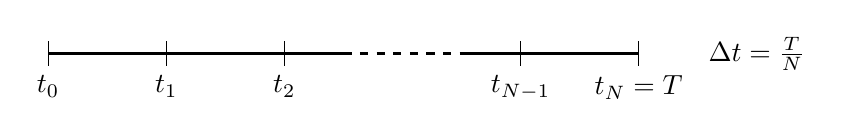
\begin{tikzpicture}[scale=1.5]
\draw[very thick] (0,0) -- (2.5,0) ;
\foreach \x in  {0,1,2}
\draw[shift={(\x,0)},color=black] (0pt,3pt) -- (0pt,-3pt);
\foreach \x in {0,1,2}
\draw[shift={(\x,0)},color=black] (0pt,0pt) -- (0pt,-3pt) node[below] 
{$t_{\x}$};
\draw[very thick,dashed] (2.5,0) -- (3.5,0) ;
\draw[very thick] (3.5,0) -- (5,0) ;
\draw[shift={(4,0)},color=black] (0pt,3pt) -- (0pt,-3pt) node [below] {$t_{N-1}$};
\draw[shift={(5,0)},color=black] (0pt,3pt) -- (0pt,-3pt) node [below] {$t_{N}=T$};
\node[color=black] at (6,0){$\Delta t = \frac{T}{N}$};
\end{tikzpicture}
\[
\begin{cases}
V(t_{N},x) = g(x)\\
V(t_{i},x) =\inf_{u\in\mathcal{U}_{t_i,t_{i+1}}}\int_{t_i}^{t_{i+1}}C(r,x_r,u_r){{\dr}}+V(t_{i+1},x_{t_{i+1}}),\\
~~~~~~~~~~~~~~~~~~~~~~~~~~~~~~~~~~~~~x_{t_{i+1}} = x + \int_{t_i}^{t_{i+1}}f(s,x_s,u_s){\ds} 
\end{cases}
\]
    \end{block}
    \begin{block}
        {Approximation}
        \[
        \begin{cases}
        \hat{V}(t_{N},x) = g(x)\\
        \hat{V}(t_{i},x):=\inf_{u}C(t_{i},x_{t_{i}},u){{\Delta t}}+\hat{V}(t_{i+1},x_{t_{i+1}}),~x_{t_{i+1}} = x + f(t_i,x,u)\Delta t 
        \end{cases}
        \]
    \end{block}
\end{frame}
%%%%%%%%%%%%%%%%%%%%%%%%%%%%%%%%%%%%%%%%
\begin{frame}{Numerical DPP}
    \begin{block}
        {Approximation}
        \[
        \begin{cases}
        \hat{V}(t_{N},x) = g(x)\\
        \hat{V}(t_{i},x):=\inf_{u}C(t_{i},x_{t_{i}},u){{\Delta t}}+\hat{V}(t_{i+1},x_{t_{i+1}}),~x_{t_{i+1}} = x + f(t_i,x,u)\Delta t 
        \end{cases}
        \]
    \end{block}
    \begin{alertblock}
        {Simplification of one-step approximate DPP}
        The  approximation is not over the control $u:[t_i,t_{i+1}]\to\mathbb{R}^m$, but over values $u\in\mathbb{R}^m$. The optimal value $\hat{u}^*$ is a constant approximately optimal control over $[t_i,t_{i+1}]$.
    \end{alertblock}
\end{frame}
%%%%%%%%%%%%%%%%%%%%%%%%%%%%%%%%%%%%%%%%
\begin{frame}{Algorithm}
    ~~~~~~~~\begin{algorithm}[H]
        % Algorithm content goes here
        \Parameter{$T$, $N$, $f(t,x,u)$, $C(t,x,u)$, and $g(x)$\;
        $\Delta t = \frac{T}{N}$}
        \KwData{$\hat{V}(t_{N},x)=g(x)$\; $x^j_i$ for $j=1,...,J$ and $i=0,...,N-1$\;
        ($x^j_i$ means the  $j$th discrete point at time $t_i$.)}
        \For{$i \leftarrow N-1$ to $0$}
        {$\hat{x}^j_{i+1}=x_i^j+f(t_{i},x_i^j,u)\Delta t$\;
        $\tilde{V}(t_{i},x^j_i)\leftarrow \inf_{u}C(t_{i},{x}^j_{i},u){{\Delta t}}+\hat{V}(t_{i+1},\hat{x}^j_{t_{i+1}})$\;
        $\hat{V}(t_{i},x)$ obtained from interpolation on $\tilde{V}(t_{i},x^j_i)$ for $j=1,...,J$\;
        $\hat{u}^*(t_i,x_i^j)\in\mathop{\text{\normalfont argmin}}\limits_{u}C(t_{i},{x}^j_{i},u){{\Delta t}}+\hat{V}(t_{i+1},\hat{x}^j_{i+1})$;
        }
        \Return{$\hat{V}(t_i,\cdot)$ and $\hat{u}^*(t_i,\cdot)$ for $i=0,...,N-1$.}
        \caption{Numerical DPP}
         \label{alg:dpp}
\end{algorithm}
\end{frame}
%%%%%%%%%%%%%%%%%%%%%%%%%%%%%%%%%%%%%%%%%%%%%%%%%
\begin{frame}{DPP algorithm}
\begin{block}
    {Exercise}
    Why interpolation is required in Algorithm~\ref{alg:dpp}? 
    
    Can we perform the algorithm by only knowing  $\hat{V}(t_{i+1},{x}^j_{i+1})$ for all $j=1,...,J$? 
    
    Note the difference between $\hat{V}(t_{i+1},{x}^j_{i+1})$ and $\hat{V}(t_{i+1},\hat{x}^j_{i+1})$ and the difference between ${x}^j_{i+1}$ and $\hat{x}^j_{i+1} = {x}^j_{i} + f(t_{i},x_{i}^j,u)\Delta t$.
    \[
    \inf_u C(t_i,x_i^j,{\color{blue}u})+\hat{V}(t_i,{x}^j_{i} + f(t_{i},x_i^j,{\color{blue}u})\Delta t)
    \]
\end{block}
\end{frame}
\begin{frame}{Quadratic example}
    \begin{block}{Example} 
Value function:
\begin{equation}
    V(t,x):= \inf_{u\in\mathcal{U}_{t}}\int_t^T\left(x_s^2+u_s^2\right){{\ds}}+\frac12x_T^2-x_T,~~~~{\dx}_s=(x_s-u_s){{\ds}}.
\end{equation}
We cannot find value functions using a myopic argument.
\end{block}
\begin{block}{Exercise}
\begin{enumerate}[label=\arabic*)]
    \item In example above, write the approximate DPP from time $t_{i}$ to $t_{i+1}$.
    \item Assume that $\hat{V}(t_{i+1},x)=a_{i+1}x^2+b_{i+1}x+c_{i+1}$ for some known values $a_{i+1}$, $b_{i+1}$, and $c_{i+1}$.
     Use  optimization of a quadratic function to find $\hat{V}(t_{i},x)$. Note that you need to use $\hat{x}_{t_{i+1}}=x+(x-u)\Delta t$.
    \item  Does $\hat{V}(t_{i},x)$ is of the form $a_{i}x^2+b_{i}x+c_{i}$? What is the relation between $(a_{i},b_{i},c_{i})$ and $(a_{i+1},b_{i+1},c_{i+1})$?
\end{enumerate}
\end{block}
\end{frame}
%%%%%%%%%%%%%%%%%%%%%%%%%%%%%%%%%%%%%%%%%%%%%%%%%
\subsection{HJ}
\begin{frame}{Hamilton-Jacobi equation}
\begin{block}
    {Hamiltonian and Lagrangian}
    Hamilton: principle of minimum action
    \begin{center}
        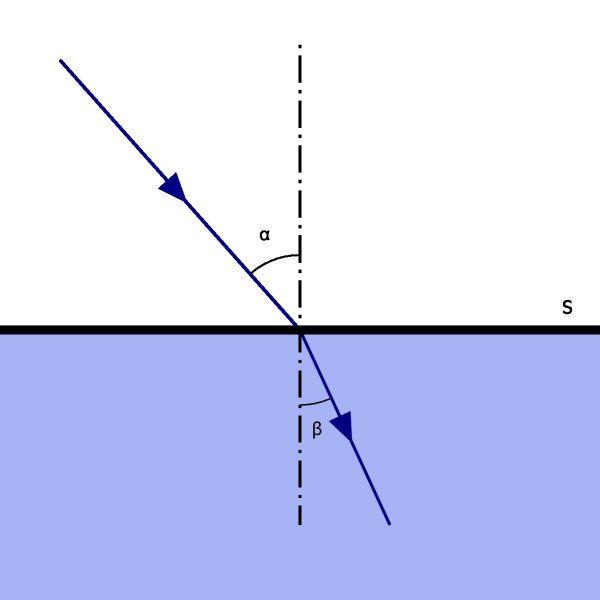
\includegraphics[width=0.4\textwidth]{Figs/Refracao.png}
    \end{center}
\end{block}
\end{frame}
%%%%%%%%%%%%%%%%%%%%%%%%%%%%%%%%%%%%%%%%
\begin{frame}{Hamilton-Jacobi equation}
    \begin{block}
        {Recall the DPP}
        \[
        V(t,x) =\inf_{u\in\mathcal{U}_{t,s}}\int_t^sC(r,x_r,{\color{blue}u_r}){{\dr}}+V(s,{\color{orange}x_s}),~~~~{\color{orange}{x}_s}=x+\int_t^sf(x_r,{\color{blue}u_r}){{\dr}}
        \]
    \end{block}
    \begin{block}
        {Taylor expansion}
        \[
V(s,{\color{orange}{x}_s}) = V(t,x) + V_t(t,x)(s-t) + V_x(t,x)({\color{orange}{x}_s}-x) + R_2
\]

\[
\begin{split}
    V(t,x) & =\inf_{u\in\mathcal{U}_{t,s}}\int_t^sC(r,x_r,u_r){{\dr}}+V(s,x_s)\\
    & = \inf_{u\in\mathcal{U}_{t,s}}\int_t^sC(r,x_r,u_r){{\dr}}\\
    & ~~~~~+V(t,x) + V_t(t,x)(s-t) + V_x(t,x)\int_t^s f(x_r,u_r){{\dr}} + R_2
\end{split}
\]
    \end{block}
\end{frame}
%%%%%%%%%%%%%%%%%%%%%%%%%%%%%%%%%%%%%%%%
\begin{frame}{Hamilton-Jacobi equation}
    \begin{block}
        {Taylor expansion}
        \[
V(s,{\color{orange}{x}_s}) = V(t,x) + V_t(t,x)(s-t) + V_x(t,x)({\color{orange}{x}_s}-x) + R_2
\]

\[
\begin{split}
    V(t,x) & =\inf_{u\in\mathcal{U}_{t,s}}\int_t^sC(r,x_r,u_r){{\dr}}+V(s,x_s)\\
    & = \inf_{u\in\mathcal{U}_{t,s}}\int_t^sC(r,x_r,u_r){{\dr}}\\
    &~~~+V(t,x) + V_t(t,x)(s-t) + V_x(t,x)\int_t^s f(x_r,u_r){{\dr}} + R_2\\
    &= V(t,x) + V_t(t,x)(s-t) +\inf_{u\in\mathcal{U}_{t,s}}\int_t^sC(r,x_r,u_r){{\dr}} \\
    &~~~+ V_x(t,x)\int_t^s f(x_r,u_r){{\dr}} + R_2
\end{split}
\]
    \end{block}
\end{frame}
%%%%%%%%%%%%%%%%%%%%%%%%%%%%%%%%%%%%%%%%
\begin{frame}{Hamilton-Jacobi equation}
    \begin{block}
        {Taylor expansion}
\[
\begin{split}
    \cancel{V(t,x)} & =\inf_{u\in\mathcal{U}_{t,s}}\int_t^sC(r,x_r,u_r){{\dr}}+V(s,x_s)\\
    &= \cancel{V(t,x)} + V_t(t,x)(s-t) +\inf_{u\in\mathcal{U}_{t,s}}\int_t^sC(r,x_r,u_r){{\dr}} \\
    &~~~+ V_x(t,x)\int_t^s f(r,x_r,u_r){{\dr}} + R_2
\end{split}
\]
Dividing both sides by $s-t$ and sending $s\to t$.
    \end{block}
\end{frame}
%%%%%%%%%%%%%%%%%%%%%%%%%%%%%%%%%%%%%%%%
\begin{frame}{Hamilton-Jacobi equation}
    \begin{block}
        {Taylor expansion}
\[
\begin{split}
    0 & =\inf_{u\in\mathcal{U}_{t,s}}\int_t^sC(r,x_r,u_r){{\dr}}+V(s,x_s)\\
    &= V_t(t,x) +\inf_{u\in\mathcal{U}_{t,s}}\lim_{s\to t}\frac{\int_t^sC(r,x_r,u_r){{\dr}}}{s-t} \\
    &~~~+ V_x(t,x)\lim_{s\to t}\frac{\int_t^s f(r,x_r,u_r){{\dr}}}{s-t} + \lim_{s\to t} \frac{R_2}{s-t}
\end{split}
\]
$R_2=o(s-t)$: $\lim_{s\to t} \frac{R_2}{s-t}=0$.
    \end{block}
\end{frame}
%%%%%%%%%%%%%%%%%%%%%%%%%%%%%%%%%%%%%%%%
\begin{frame}{Hamilton-Jacobi equation}
    \begin{block}
        {HJ equation}
\[
\begin{split}
    0 & = V_t(t,x) +\inf_{u}\Big\{C(t,x,u) + V_x(t,x)  f(t,x,u) \Big\}
\end{split}
\]
\[
\begin{cases}
    0  = V_t(t,x) + H(t,x,V_x(t,x))\\
    V(T,x)=g(x)
\end{cases}
\]
Hamiltonian: 
$H(t,x,p)= \inf_{u}\Big\{C(t,x,u) + p\cdot   f(t,x,u) \Big\}$
    \end{block}
\end{frame}
%%%%%%%%%%%%%%%%%%%%%%%%%%%%%%%%%%%%%%%%
\begin{frame}{LQC}
    \begin{block}
        {A linear-quadratic control problem}
        Consider the control problem:
\begin{equation}
\inf_{u}\bigg\{\int_0^T\Big(x_t^2 +u_t^2\Big) {{\dt}}\bigg\},~~~{\dx}_t = (-\beta x_t + u_t ){{\dt}}
\end{equation}
$C(t,x,u)=x^2 + u^2$ and $f(t,x,u)=-\beta x + u$.

Write the HJ  equation. 

After writing the HJ, plug in $V(t,x)=a(t)x^2+b(t)x+c(t)$the HJ and find ODEs for $a(t)$, $b(t)$, and $c(t)$. What are $a(T)$, $b(T)$, and $c(T)$?
    \end{block}
\end{frame}
%%%%%%%%%%%%%%%%%%%%%%%%%%%%%%%%%



\begin{frame}{Eikonal equation}
    \begin{block}
        {Fastest exit}
        Recall the fastest exit problem.
        \[
        \inf_u\int_0^\infty \mathds{1}_{\{x_t\in D\}}{\dt},~{\dx}_t=u_t{{\dt}}~\text{ with }~|u_t|\le1
        \]
        
        Write the definition of value function for initial state $x_0=x\in D$. Write the HJ equation. 
        Is there any boundary condition?
    \end{block}
% \end{frame}
% %%%%%%%%%%%%%%%%%%%%%%%%%%%%%%%%%%%%%%%%

% \begin{frame}{Eikonal equation}
    \begin{block}
        {Solution to Eikonal equation}
        Write the HJ equation and boundary condition for the special case where $D=[-1,1]\subset\mathbb{R}$. Which one of the following functions satisfy the HJ equation? Which one matches the value function?
        \[
        v_1(x) = 1-|x|, v_2(x)= \begin{cases}
            \frac12-|x-\frac12|&0\le x\le1\\
            \frac12-|x+\frac12|&-1\le x<0
        \end{cases}
        \]
    \end{block}
\end{frame}
%%%%%%%%%%%%%%%%%%%%%%%%%%%%%%%%%%%%%%%%

\begin{frame}{SIR model in epidemiology}
    \begin{block}
        {ODEs}
        Susceptible, infected, and recovered:
        \[
        \begin{cases}
            \dd{S}_t=-\beta S_t I_t \dt\\
            \dd{I}_t = (\beta I_t S_t - \gamma I_t)\dt\\
            \dd{R}_t= \gamma I_t \dt
        \end{cases}
        \]
    \end{block}
    \begin{block}
        {Controlled state variables}
        Susceptible, infected, and recovered:
        \[
        \begin{cases}
            \dd{S}_t=-\beta_t S_t I_t \dt\\
            \dd{I}_t = (\beta_t I_t S_t - \gamma_t I_t)\dt\\
            \dd{R}_t= \gamma_t I_t \dt
        \end{cases}
        \]
        $\beta_t\in[b_0,b_1]$ and $\gamma_t\in[c_0,c_1]$ all positive.
    \end{block}
\end{frame}


%%%%%%%%%%%%%%%%%%%%%%%%%%%%%%%%%%%


\begin{frame}{SIR model in epidemiology}
    \begin{block}
        {Controlled state variables}
        Susceptible, infected, and recovered:
        \[
        \begin{cases}
            \dd{S}_t=-\beta_t S_t I_t \dt\\
            \dd{I}_t = (\beta_t I_t S_t - \gamma_t I_t)\dt\\
            \dd{R}_t= \gamma_t I_t \dt
        \end{cases}
        \]
        $\beta_t\in[b_0,b_1]$ and $\gamma_t\in[c_0,c_1]$ all positive.
    \[
    \inf_{\beta_t,\gamma_t}\int_0^T ((b_1-\beta_t)^2+\gamma_t^2)\dt + I^2_T
    \]
    Write the HJ equation in variables $x=(S,I,R)$.
    \end{block}
\end{frame}
%%%%%%%%%%%%%%%%%%%%%%%%%%%%%%%%%

\begin{frame}{SIR model in epidemiology}
    \begin{block}
        {Controlled state variables}
        Susceptible, infected, and recovered:
        \[
        \begin{cases}
            \dd{S}_t=-\beta_t S_t I_t \dt\\
            \dd{I}_t = (\beta_t I_t S_t - \gamma_t I_t)\dt\\
            \dd{R}_t= \gamma_t I_t \dt
        \end{cases}
        \]
        $\beta_t\in[b_0,b_1]$ and $\gamma_t\in[c_0,c_1]$ all positive.
    \[
    \inf_{\beta_t,\gamma_t}\int_0^T ((b_1-\beta_t)^2+\gamma_t^2)\dt + I^2_T
    \]
    Notice that $\dd(S_t+I_t+R_t)=0$. This should allow us to reduce the number of state variables $x_t=(S_t,I_t,R_t)$ to two, in place of three. Assume that the population size is given by $N$, $S_t+I_t+R_t=N$. Remove the variable $R_t$ and write the HJ equation in terms of $(S_t,I_t)$.
    Write the HJ equation in $(S,I)$.
    \end{block}
\end{frame}

%%%%%%%%%%%%%%%%%%%%%%%%%%%%%%%%%

\begin{frame}{Consumption}
    \begin{block}
        {Savings account}
        \[
        \dd{x}_t = (rx_t - c_t)\dt
        \]
        $c_t\ge0$ is the rate of consumption.
        \[
        \sup_{c_t\ge0} \int_0^T U(c_t)\dt + U(x_T)
        \]
        $U$ is a given function called {\color{blue}utility function}.
    \end{block}
\end{frame}

%%%%%%%%%%%%%%%%%%%%%%%%%%%%%%%%%

\begin{frame}{Consumption}
    \begin{block}
        {Utility function}
        Utility function is a concave function that represent our enjoyment from consumption or wealth. The concavity signifies the fact that if our consumption or wealth level is low, increasing one more unit grants more joy compared to when our consumption or wealth level is higher and we obtain one more unit.
        Example of a utility function:
        \begin{center}
            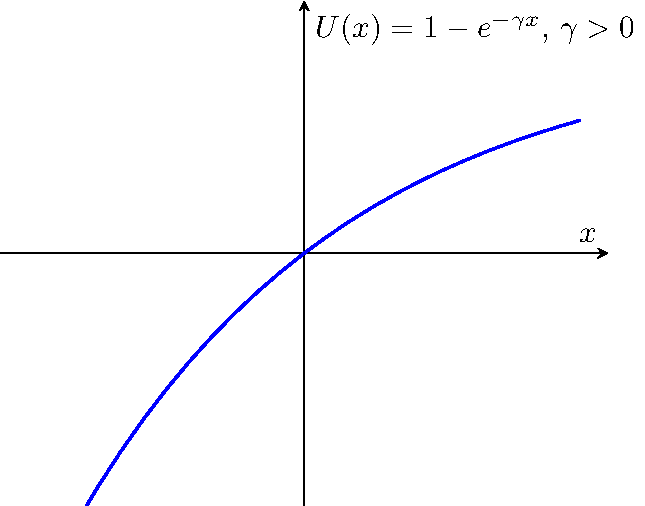
\includegraphics[width=0.35\linewidth]{Control_lecture_notes/Figs/utility1.pdf}
            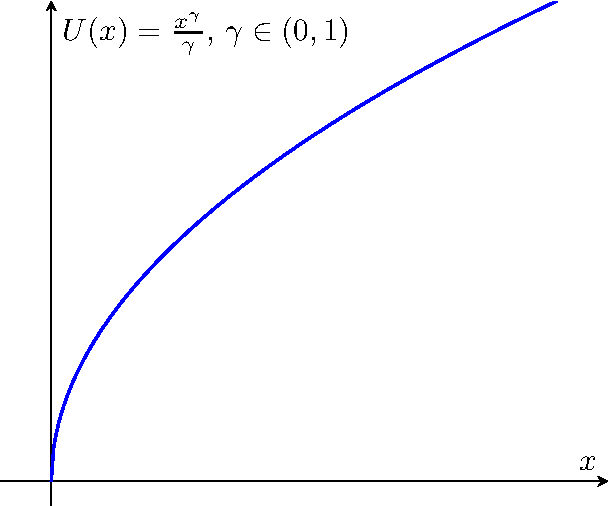
\includegraphics[width=0.35\linewidth]{Control_lecture_notes/Figs/utility2.pdf}
        \end{center}
        
    \end{block}
\end{frame}

%%%%%%%%%%%%%%%%%%%%%%%%%%%%%%%%%

\begin{frame}{Consumption}
    \begin{block}
        {Savings account}
        \[
        \dd{x}_t = (rx_t - c_t)\dt
        \]
        $c_t\ge0$ is the rate of consumption.
        \[
        \sup_{c_t\ge0} \int_0^T U(c_t)\dt + U(x_T)
        \]
        HJ equation is given by:
        \[
        \begin{cases}
            V_t+H(x,V_x)=0\\
            V(T,x)=U(x)
        \end{cases}
        \]
        with $H(x,p)=\sup_{c\ge0}\{U(x)-cp\}+rxp$
    \end{block}
\end{frame}

%%%%%%%%%%%%%%%%%%%%%%%%%%%%%%%%%
\begin{frame}{Solving HJ equation for consumption}
\begin{block}
    {Utility $U(c)=\frac{c^{\gamma}}{\gamma}$ for $c\ge0$}
    Show that the supremum in Hamiltonian is attained at $c^*(p)=p^{\frac{1}{\gamma-1}}$ and
    \[
        H(x,p)=\sup_{c\ge0}\Bigg\{\frac{c^{\gamma}}{\gamma}-cp\Bigg\}+rxp=\frac{1-\gamma}{\gamma}
        p^{\frac{1}{\gamma-1}}+rxp
    \]
    Verify that  $V(t,x)=f(t)\frac{c^{\gamma}}{\gamma}$ solves the HJ equation 
    \[
    \begin{cases}
        0=V_t+V_x^{\frac{\gamma}{\gamma-1}}+rxV_x\\
        V(T,x)=\frac{c^{\gamma}}{\gamma}
    \end{cases}
    \]
    and $f(t)$ satisfies
    \[
    \begin{cases}
        0=f^{\prime}+f^{\frac{\gamma}{\gamma-1}}+\frac{r}{\gamma}f\\
        f(T)=1
    \end{cases}
    \]
\end{block}
\end{frame}
%%%%%%%%%%%%%%%%%%%%%%%%%%%%%%%%%
\begin{frame}{Solving HJ equation for consumption}
\begin{block}
    {Utility $U(c)=\frac{c^{\gamma}}{\gamma}$ for $c\ge0$}
    We solve the ODE
    $0=f^{\prime}+f^{\frac{\gamma}{\gamma-1}}+\frac{r}{\gamma}f$
    by the change of variable $f = y^{1-\gamma}$. 
    
    $y$ satisfies $y' + \frac{r}{\gamma(1-\gamma)} y + \frac{1}{1-\gamma} = 0$ and  $y(t) = \Big(1+\frac{\gamma}{r}\Big) e^{\frac{r}{\gamma(1-\gamma)}(T-t)} - \frac{\gamma}{r}$. 
    \[
    f(t)=\Bigg(\Big(1+\frac{\gamma}{r}\Big) e^{\frac{r}{\gamma(1-\gamma)}(T-t)} - \frac{\gamma}{r}\Bigg)^{1-\gamma}
    \]
    Since $1-\gamma<0$, $f(t)>1$ unless $t=T$. The optimal consumption $c^*(t,x)=\frac{1}{f^{\frac{1}{1-\gamma}}(t)}x$ or
    \[
    \begin{cases}
       c^*_t=\frac{1}{f^{\frac{1}{1-\gamma}}(t)}x_t\\
       \dx_t = \Big(r - \frac{1}{f^{\frac{1}{1-\gamma}}(t)}\Big)x_t\dt
    \end{cases}
    \]
\end{block}
\end{frame}
%%%%%%%%%%%%%%%%%%%%%%%%%%%%%%%%%

\begin{frame}{Solving HJ equation for consumption}
\begin{block}
    {Utility $U(c)=\frac{c^{\gamma}}{\gamma}$ for $c\ge0$} 
    \[
    \begin{cases}
       c^*_t=\frac{1}{f^{\frac{1}{1-\gamma}}(t)}x_t\\
       \dx_t = \bigg(r - \frac{1}{f^{\frac{1}{1-\gamma}}(t)}\bigg)x_t\dt
    \end{cases}
    \]
We learn from the above solution that $\frac{1}{f^{\frac{1}{1-\gamma}}(t)}<1$, therefore the optimal consumption rate percentage of wealth and the account balance never goes negative.
\end{block}

\begin{block}
    {Coding exercise}
    Plot the solution of 
    $\dx_t = \bigg(r - \frac{1}{f^{\frac{1}{1-\gamma}}(t)}\bigg)x_t\dt$
    for different values for $r>0$, $\gamma\in(0,1)$, $T$, and different initial balance $x>0.$
\end{block}

\end{frame}
%%%%%%%%%%%%%%%%%%%%%%%%%%%%%%%%%


\begin{frame}{Consumption with no terminal wealth}
    \begin{block}
        {Savings account}
        \[
        \dd{x}_t = (rx_t - c_t)\dt
        \]
        $c_t\ge0$ is the rate of consumption.
        \[
        \sup_{c_t\ge0} \int_0^T U(c_t)\dt \cancel{+ U(x_T)}
        \]
        Can we consume infinitely by borrowing? 
.
        If we restrict consumption to case where borrowing is not allowed, $x_t\ge0$ for all $t$, does this solve the issue? (Relation to admissible control.)

        Write the HJ equation with boundary condition that reflects $x_t\ge0$.
    \end{block}
\end{frame}

%%%%%%%%%%%%%%%%%%%%%%%%%%%%%%%%%

\begin{frame}{Consumption with decay}
    \begin{block}
        {Savings account}
        \[
        \dd{x}_t = (rx_t - c_t)\dt
        \]
        $c_t\ge0$ is the rate of consumption.
        \[
        \sup_{c_t\ge0} \int_0^T {\color{orange}e^{-kt}}U(c_t)\dt + {\color{orange}e^{-kT}}U(x_T)
        \]
        Write the HJ equation. Hint: $C(t,x,u)={\color{orange}e^{-kt}}U(u)$
    \end{block}
\end{frame}

%%%%%%%%%%%%%%%%%%%%%%%%%%%%%%%%%

\begin{frame}{Dynamic programming equation with decay}
    \begin{block}
        {Control problem with decay}
        \[
        \inf_{u}\int_0^T {\color{orange}e^{-kt}}\bar{C}(x_t,u_t)\dt+{\color{orange}e^{-kT}}g(x_T),~~~~\dx_t = f(x_t,u_t)\dt
        \]
    \end{block}
    \begin{block}
        {Value function}
        \[
        V(t,x):=\inf_{u}\int_t^T {\color{orange}e^{-k(s-t)}}\bar{C}(x_s,u_s)\ds + {\color{orange}e^{-k(T-t)}}g(x_T)
        \]
    \end{block}
    \begin{block}
        {DPP}
        \[
        V(t,x)=\inf_{u}\int_t^s {\color{orange}e^{-k(r-t)}}\bar{C}(x_r,u_r)\dr + {\color{orange}e^{-k(s-t)}}V(s,x_s)
        \]
    \end{block}
\end{frame}
%%%%%%%%%%%%%%%%%%%%%%%%%%%%%%%%%

\begin{frame}{Dynamic programming equation with decay}
    \begin{block}
        {Value function}
        \[
        V(t,x):=\inf_{u}\int_t^T {\color{orange}e^{-k(s-t)}}\bar{C}(x_s,u_s)\ds + {\color{orange}e^{-k(T-t)}}g(x_T)
        \]
    \end{block}
    \begin{block}
        {DPP}
        \[
        V(t,x)=\inf_{u}\int_t^s {\color{orange}e^{-k(r-t)}}\bar{C}(x_r,u_r)\dr + {\color{orange}e^{-k(s-t)}}V(s,x_s)
        \]
    \end{block}
        \begin{block}
        {HJB with decay}
        Write the first three terms of the Taylor polynomial for ${\color{orange}e^{-k(s-t)}}V(s,x_s)$ about point $(t,x)$.
    \end{block}
\end{frame}
%%%%%%%%%%%%%%%%%%%%%%%%%%%%%%%%%

\begin{frame}{Dynamic programming equation with decay}
        \begin{block}
        {HJB with decay}
        \[
        \begin{split}
             {\color{orange}e^{-k(s-t)}}V(s,x_s) = &V(t,x) + \Big(\big(V_t(t,x) {\color{orange}- k V(t,x)}\big)(s-t)\\
             &~~~~+ V_x(t,x)\int_t^s f(x_r,u_r)\dr\Big) + O((s-t)^2)
        \end{split}
        \]
        \[
        \begin{split}
            \cancel{V(t,x)}=\inf_{u}\int_t^s &{\color{orange}e^{-k(r-t)}}\bar{C}(x_r,u_r)\dr \\
            &+ \cancel{V(t,x)} + \Big(\big(V_t(t,x) {\color{orange}- k V(t,x)}\big)(s-t)\\
             &~~~~+ V_x(t,x)\int_t^s f(x_r,u_r)\dr\Big) + O((s-t)^2)
        \end{split}
        \]
    \end{block}
\end{frame}
%%%%%%%%%%%%%%%%%%%%%%%%%%%%%%%%%

\begin{frame}{Dynamic programming equation with decay}
        \begin{block}
        {HJB with decay}
        Divide by $s-t$ and $s\to t$:
        \[
        \begin{split}
            0=\inf_{u} &\bar{C}(x,u) + V_t(t,x) {\color{orange}- k V(t,x)}+ V_x(t,x)\cdot f(x,u)
        \end{split}
        \]
        \[
        \begin{split}
            0= V_t(t,x) {\color{orange}- k V(t,x)}+\inf_{u} &\{\bar{C}(x,u) + V_x(t,x)\cdot f(x,u)\}
        \end{split}
        \]
        Hamiltonian: 
        \[
        H(x,p):= \inf_{u} \{\bar{C}(x,u) + p\cdot f(x,u)\}
        \]
    \end{block}
\end{frame}
%%%%%%%%%%%%%%%%%%%%%%%%%%%%%%%%%
\begin{frame}{Purpose of different HJ for decay}
    \begin{block}
        {Infinite horizon}
        Time-homogeneity
        \[
        V(x)=\inf_{u}\int_t^\infty {\color{orange}e^{-k(s-t)}}\bar{C}(x_s,u_s)\ds=\inf_{u}\int_0^\infty {\color{orange}e^{-ks}}\bar{C}(x_s,u_s)\ds
        \]
    \end{block}
    \begin{block}
        {HJ equation}
        \[
        \begin{split}
            0= {\color{orange}- k V(x)}+\inf_{u} &\{\bar{C}(x,u) + V_x(x)f(x,u)\}
        \end{split}
        \]
    \end{block}
\end{frame}
%%%%%%%%%%%%%%%%%%%%%%%%%%%%%%%%%

\begin{frame}{Consumption with decay}
    \begin{block}
        {Savings account}
        $\dd{x}_t = (rx_t - c_t)\dt$.
        $c_t\ge0$ is the rate of consumption.
        \[
        \sup_{c_t\ge0} \int_0^\infty {\color{orange}e^{-kt}}U(c_t)\dt
        \]
        where consumption strategy must satisfy $x_t\ge0$ for all $t\ge0$.
        Write the HJ equation with proper boundary condition. Solve the HJ equation for $U(c)=\frac{c^\gamma}{\gamma}$ for $\gamma\in(0,1)$. Hint: find a constant $f$ such that $V(x)=f\frac{x^\gamma}{\gamma}$ solves the HJ equation. Is the optimal consumption a constant multiple of $x$?
    \end{block}
    \begin{block}
    {Coding exercise}
        Plot optimal wealth 
        $\dx_t = \bigg(r - c^*\bigg)x_t\dt$
        for different values for $r>0$, $\gamma\in(0,1)$, and different initial balance $x>0.$
\end{block}
\end{frame}
%%%%%%%%%%%%%%%%%%%%%%%%%%%%%%%%%%%%%%%%
\begin{frame}{Summary of HJ method}
    \begin{figure}
        \centering
        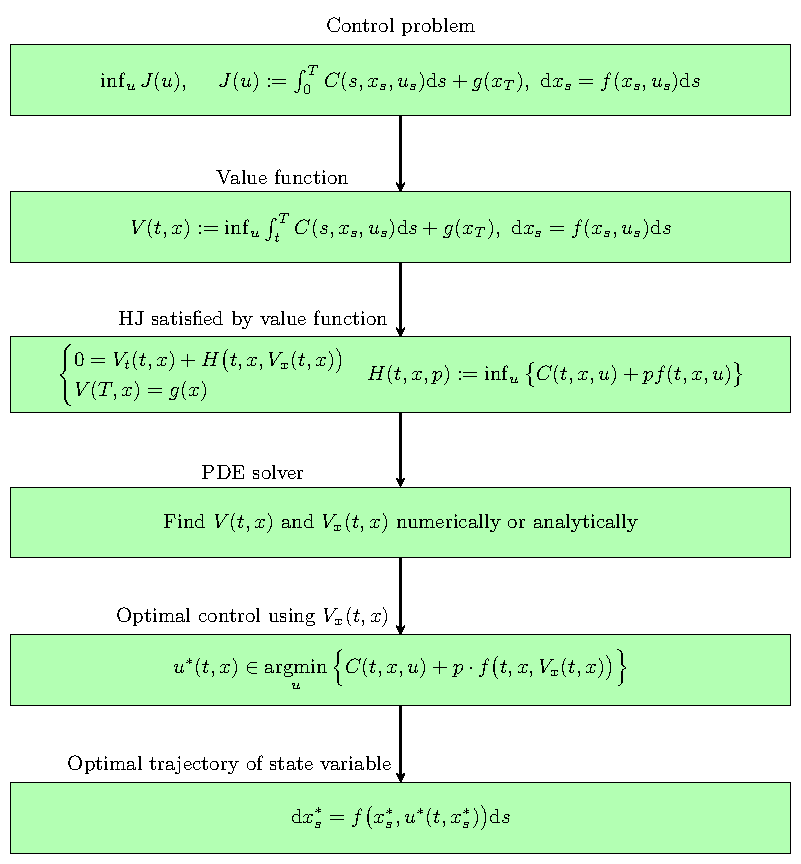
\includegraphics[height=0.75\textheight]{Control_lecture_notes/Figs/HJ_chart.pdf}
    \end{figure}
\end{frame}

%%%%%%%%%%%%%%%%%%%%%%%%%%%%%%%%%%%%%%%%
%%%%%%%%%%%%%%%%%%%%%%%%%%%%%%%%%%%%%%%%
%%%%%%%%%%%%%%%%%%%%%%%%%%%%%%%%%%%%%%%%
%%%%%%%%%%%%%%%%%%%%%%%%%%%%%%%%%%%%%%%%
\section{Lagrange multiplier}
\begin{frame}{Lagrange multiplier}
    \begin{block}
        {Constrained optimization}
        \[
        \inf_x f(x) ~~~ \textrm{subject to}~~~g(x)=0
        \]
    \end{block}
    \begin{block}
        {Lagrangian}
        \[
        L(x,\lambda):= f(x) - \lambda \cdot g(x)
        \]
    \end{block}
    \begin{block}
        {Saddle point problem}
        \[
        \sup_{\lambda}\inf_{x}L(x,\lambda)=\sup_{\lambda}H(\lambda)
        \]
        with $H(\lambda):=\inf_{x}L(x,\lambda)$ called Hamiltonian.
    \end{block}
\end{frame}
%%%%%%%%%%%%%%%%%%%%%%%%%%%%%%%%%%%%%%%%
\begin{frame}{Lagrange multiplier}
    \begin{block}
        {Saddle point problem}
        \[
        \sup_{\lambda}\inf_{x}L(x,\lambda)
        \]
    \end{block}
        \begin{block}
        {Strong duality}
        If 
        $\sup_{\lambda}\inf_{x}L(x,\lambda) =\inf_{x}\sup_{\lambda}L(x,\lambda)$
        holds, we call it strong duality.
        \[
        \begin{split}
            \inf_{x}\sup_{\lambda}L(x,\lambda)= \inf_{x}\sup_{\lambda}f(x)-\lambda\cdot g(x)= \inf_{x}f(x)-\inf_{\lambda}\lambda \cdot g(x)
        \end{split}
        \]
        If at a point $x$, $g(x)\neq0$, then $\inf_{\lambda}\lambda \cdot g(x)=-\infty$. Therefore, $x$ is not a saddle point.
    \end{block}
\end{frame}
%%%%%%%%%%%%%%%%%%%%%%%%%%%%%%%%%%%%%%%%
\begin{frame}{Geometric interpretation of Lagrange multiplier}
    \begin{figure}
        \centering
        \includesvg[scale=0.42]{LagrangeMultipliers2D.svg}
        \caption{At the infimum point, $\nabla f$ and $\nabla g$ are parallel, $\nabla f=\lambda\nabla g$.}
        \label{fig:Lagrange}
    \end{figure}
\end{frame}
%%%%%%%%%%%%%%%%%%%%%%%%%%%%%%%%%%%%%%%%
\begin{frame}{Karush-Kuhn-Tucker (KKT) condition}
    \begin{block}
        {KKT}
        Assume the differentiability of $f$ and $g$.
    If $x^*$ solves $\inf_x f(x)$   subject to $g(x)=0$ and $\lambda^*$ solves $\sup_{\lambda}H(\lambda)$ such that 
    \begin{equation} \label{cond:KKT}
    \begin{cases} \triangledown f(x^*) - \lambda^* \cdot \triangledown g(x^*) = 0\\
            g (x^*)=0
        \end{cases}
    \end{equation}
    then, strong duality holds and $(x^*,\lambda^*)$ is a saddle point for $\sup_{\lambda}\inf_{x}L(x,\lambda)$. 

    Conversely, if strong duality holds, then any saddle point $(x^*,\lambda^*)$ satisfies \eqref{cond:KKT}. 
    In particular, $x^*$ solve 
    \[
        \inf_x f(x) ~~~ \textrm{subject to}~~~g(x)=0
    \]
    \end{block}
\end{frame}
%%%%%%%%%%%%%%%%%%%%%%%%%%%%%%%%%%%%%%%%
\begin{frame}{Constrained optimal control problem}
\begin{block}
    {Simple example}
    \[
        \inf_{u}\int_0^T\Big(x_t^2 - \alpha_t x_t\Big) {{\dt}}
    \]
    where $\dx_t=u_t\dt$ subject to $\int_0^Tx_t\dt = 0$.
    Lagrangian
    \[
    L(u,\lambda):=\int_0^T\Big(x_t^2 - \alpha_t x_t\Big) {{\dt}}-\lambda\int_0^Tx_t\dt =  \int_0^T\Big(x_t^2 - (\alpha_t + \lambda) x_t\Big) {{\dt}}
    \]
    Myopic solution with KKT:
    \[
    x^*_t =   (\alpha_t + \lambda^* )/2~~\text{ and }~~\int_0^Tx^*_s\ds = 0
    \]
    Therefore,
    \[
    \lambda^*=-\frac1T\int_0^T\alpha_s\ds~~\text{ and }~~x^*_t =   \frac{\alpha_t - \frac{1}{T}\int_0^T\alpha_s{{\ds}}}{2}
    \]
\end{block}
    
\end{frame}
%%%%%%%%%%%%%%%%%%%%%%%%%%%%%%%%%%%%%%%%
\section{Pontryagin principle}
\begin{frame}{Pontryagin principle: real application of Lagrange multiplier}
    \begin{block}
        {What is the constraint?}
    \begin{equation}
        \inf_{u}\bigg\{\int_0^T\Big(x_t^2 - \alpha_t x_t\Big) {{\dt}}+x_T^2\bigg\}
    \end{equation}
    Constraint: {\color{orange}${\dx}_t = (-\beta x_t + u_t ){{\dt}}$}
    \end{block}
    \begin{block}
        {Lagrangian}
        \[
        L(u,\lambda)= \int_0^T\Big(x_t^2 - \alpha_t x_t\Big) {{\dt}} +x_T^2 - {\color{orange}\int_0^T \lambda_t\cdot({\dx}_t-(-\beta x_t + u_t ){{\dt}})}
        \]
        
    \end{block}
    \begin{block}
        {Integration by parts}
        Apply integration by parts on 
        ${\color{orange}\int_0^T \lambda_t\cdot{\dx}_t}$
        and substitute it into Lagrangian.
    \end{block}
\end{frame}
%%%%%%%%%%%%%%%%%%%%%%%%%%%%%%%%%%%%%%%%
\begin{frame}{Pontryagin principle: real application of Lagrange multiplier}
    \begin{block}
        {Simplify Lagrangian}
        Integration by parts
    \[
    \int_0^T \lambda_t\cdot {\dx}_t = \lambda_Tx_T-\lambda_0x_0-\int_0^T x_t\cdot {\dd}\lambda_t
    \]
        \[
        \begin{split}
        L(u,\lambda)=& \int_0^T\Big(x_t^2 - \alpha_t x_t\Big) {{\dt}}+x_T^2 \\
        &~~- \Big(\lambda_Tx_T-\lambda_0x_0 -\int_0^T x_t\cdot({\dd}\lambda_t-(-\beta x_t + u_t ){{\dt}})\Big)  \\
        =& \int_0^T\Big(\big(x_t^2 - \alpha_t x_t -x_t\cdot(-\beta x_t + u_t)\big)\dt + x_t\cdot{\dd}\lambda_t  \Big) \\
        &~~+ x_T^2- \lambda_Tx_T +\lambda_0 x_0
        \end{split}\]
        
    \end{block}
\end{frame}
%%%%%%%%%%%%%%%%%%%%%%%%%%%%%%%%%%%%%%%%
\begin{frame}{Pontryagin principle: real application of Lagrange multiplier}
    \begin{block}
        {Hamiltonian (new)}
        \[
        \begin{split}
        L(u,\lambda)=& \int_0^T\Big(\big({\color{orange}x_t^2 - \alpha_t x_t -x_t\cdot(-\beta x_t + u_t})\big)\dt + x_t\cdot{\dd}\lambda_t  \Big) \\
        &~~+ x_T^2- \lambda_Tx_T +\lambda_0 x_0
        \end{split}\]
        $H(t,x,\lambda,u)={\color{orange}x^2 - \alpha_t x -x\cdot\big(-\beta x + u)}$
    \end{block}
    \begin{block}
        {Myopically perform KKT}
        Minimizing $x_T^2- \lambda_Tx_T$ wrt $x_T$: $\lambda^*_T=2x^*_T$\\
        Minimizing Hamiltonian wrt $u$: $H(t,x^*_t,\lambda^*_t,u^*_t)=\inf_{u}H(t,x^*_t,\lambda^*_t,u)$
        Minimizing integrand wrt $x_t$: 
        \[
        \dd\lambda^*_t + H_x(t,x^*_t,\lambda^*_t,u^*_t)=0
        \]
    \end{block}
\end{frame}
%%%%%%%%%%%%%%%%%%%%%%%%%%%%%%%%%%%%%%%%
\begin{frame}{Putting all together}
    \begin{block}
        {Pontriagyn maximum principle}
        If we can find functions $x^*_t$, $\lambda^*_t$, and $u^*_t$ such that 
    \[
    \begin{cases}
        {\dd}\lambda^*_t+ \partial_x H(t,x^*_t,\lambda^*_t,u^*_t){{\dt}}={\dd}\lambda^*_t+ (-\lambda^*_t \beta  +2x^*_t -\alpha_t){{\dt}}=0\\
        \hspace{7cm}(\textrm{minimize integrand wrt $x$})\\
        \lambda^*_T=2x_T^* ~(\textrm{minimize terminal wrt $x_T$})\\
        H(t,x^*_t,\lambda^*_t,u^*_t)\le H(t,x^*_t,\lambda^*_t,u)~\textrm{ for all } u ~(\textrm{minimize integrand wrt $u$})\\
        {\dx}^*_t = (-\beta x^*_t + u^*_t) {{\dt}} ~(\textrm{constraint})
        \end{cases}
    \]
    Then, $u^*_t$ is an optimal control and $x^*_t$ is an optimal trajectory.
    \end{block}
\end{frame}
%%%%%%%%%%%%%%%%%%%%%%%%%%%%%%%%%%%%%%%%
\begin{frame}{General case}
    \begin{block}
        {Pontriagyn maximum principle}
        Define
        \[
        H(t,x,\lambda,u) := C(t,x,u)-\lambda\cdot f(t,x,u)
        \]
        If we can find functions $x^*_t$, $\lambda^*_t$, and $u^*_t$ such that 
    \[
    \begin{cases}
        {\dd}\lambda^*_t+ \partial_x H(t,x^*_t,\lambda^*_t,u^*_t){{\dt}}=0,~(\textrm{minimize integrand wrt $x$})\\
        \lambda^*_T=g_x(x_T^*) ~(\textrm{minimize terminal wrt $x_T$})\\
        H(t,x^*_t,\lambda^*_t,u^*_t)\le H(t,x^*_t,\lambda^*_t,u)~\textrm{ for all } u ~(\textrm{minimize integrand wrt $u$})\\
        {\dx}^*_t = f(t,x^*_t,u^*_t) {{\dt}} ~(\textrm{constraint})
        \end{cases}
    \]
    Then, $u^*_t$ is an optimal control and $x^*_t$ is an optimal trajectory.
    \end{block}
\end{frame}
\begin{frame}{Pontriagyn maximum principle}

\begin{block}
    {Relation between Pontriagyn principle and value function}
    If the value function is differentiable and the condition of Pontriagyn principle holds, then
    \[
    \lambda^*_t=V_x(t,x^*_t)
    \]
\end{block}
\begin{block}
    {Example}
    Write Pontriagyn maximum principle for the control problem with 
    \[
     \inf_{u}\int_0^T(x_t^2 + u_t^2 ){{\dt}} + x^2_T + x_T,~\text{ subject to  }~{\dx}_t=( x_t +  u_t){{\dt}}
    \]
    Can you solve the equations and find $x^*$, $\lambda^*$, and $u^*$?
\end{block}
    
\end{frame}
%%%%%%%%%%%%%%%%%%%%%%%%%%%%%%%%%%%%%%%%
%%%%%%%%%%%%%%%%%%%%%%%%%%%%%%%%%%%%%%%%
%%%%%%%%%%%%%%%%%%%%%%%%%%%%%%%%%%%%%%%%
%%%%%%%%%%%%%%%%%%%%%%%%%%%%%%%%%%%%%%%%
\begin{frame}{Individual project}
\begin{block}{Due end October}
     In your area of study, find an optimal control problem. Then, write the cost functions and the control variable and determine a set of admissible controls. 
\end{block}
\end{frame}

%%%%%%%%%%%%%%%%%%%%%%%%%%%%%%%%%%%%%%%%
%%%%%%%%%%%%%%%%%%%%%%%%%%%%%%%%%%%%%%%%
%%%%%%%%%%%%%%%%%%%%%%%%%%%%%%%%%%%%%%%%
%%%%%%%%%%%%%%%%%%%%%%%%%%%%%%%%%%%%%%%%
\section{Stochastic control}
\begin{frame}{Noise}
    \begin{block}
        {Observations are often noisy!}
        
\includegraphics[scale=.3]{Control_lecture_notes/Figs/rf.jpg}
    \end{block}
\end{frame}
\begin{frame}{Noise}
    \begin{block}
        {Observations are often noisy!}
        Fantasy: $\dX_t=b(t,X_t,u_t)\dt$

        Real world: $\dX_t=b(t,X_t,u_t)\dt+\text{noise}$
    \end{block}
    \begin{block}{white noise} Denoted by $\dW_t$, at two different times $t_1$ and $t_2$, $\dW_{t_1}$ and $\dW_{t_2}$ are independent.

        To many's disappointment, white noise does not exist in a conventional sense. \textbf{\emph{Brownian motion}, a.k.a. \emph{Wiener process} describes the noise}
    \end{block}
\end{frame}
\begin{frame}{Stochastic}
\begin{block}{Stochastic process}
A stochastic process $\{X_t\}_{t}$ is a set of random variables indexed by time $t\in[0,\infty)$. It represents evolution of an uncertain quantity over time. At each time $t$, $X_t$ is a random variable with a certain distribution that depends on $t$. Furthermore, the joint distribution of $X_{t_1},...,X_{t_n}$ for different times $t_1,...,t_n$ is important in shaping a stochastic process.

An observation, denoted by $\omega$, is one \emph{realization} of a stochastic process. The function $X(\omega):[0,\infty)\to\mathbb{R}^d$ is called a sample path of $X$.
\end{block}
    
\end{frame}
\begin{frame}{Stochastic}
    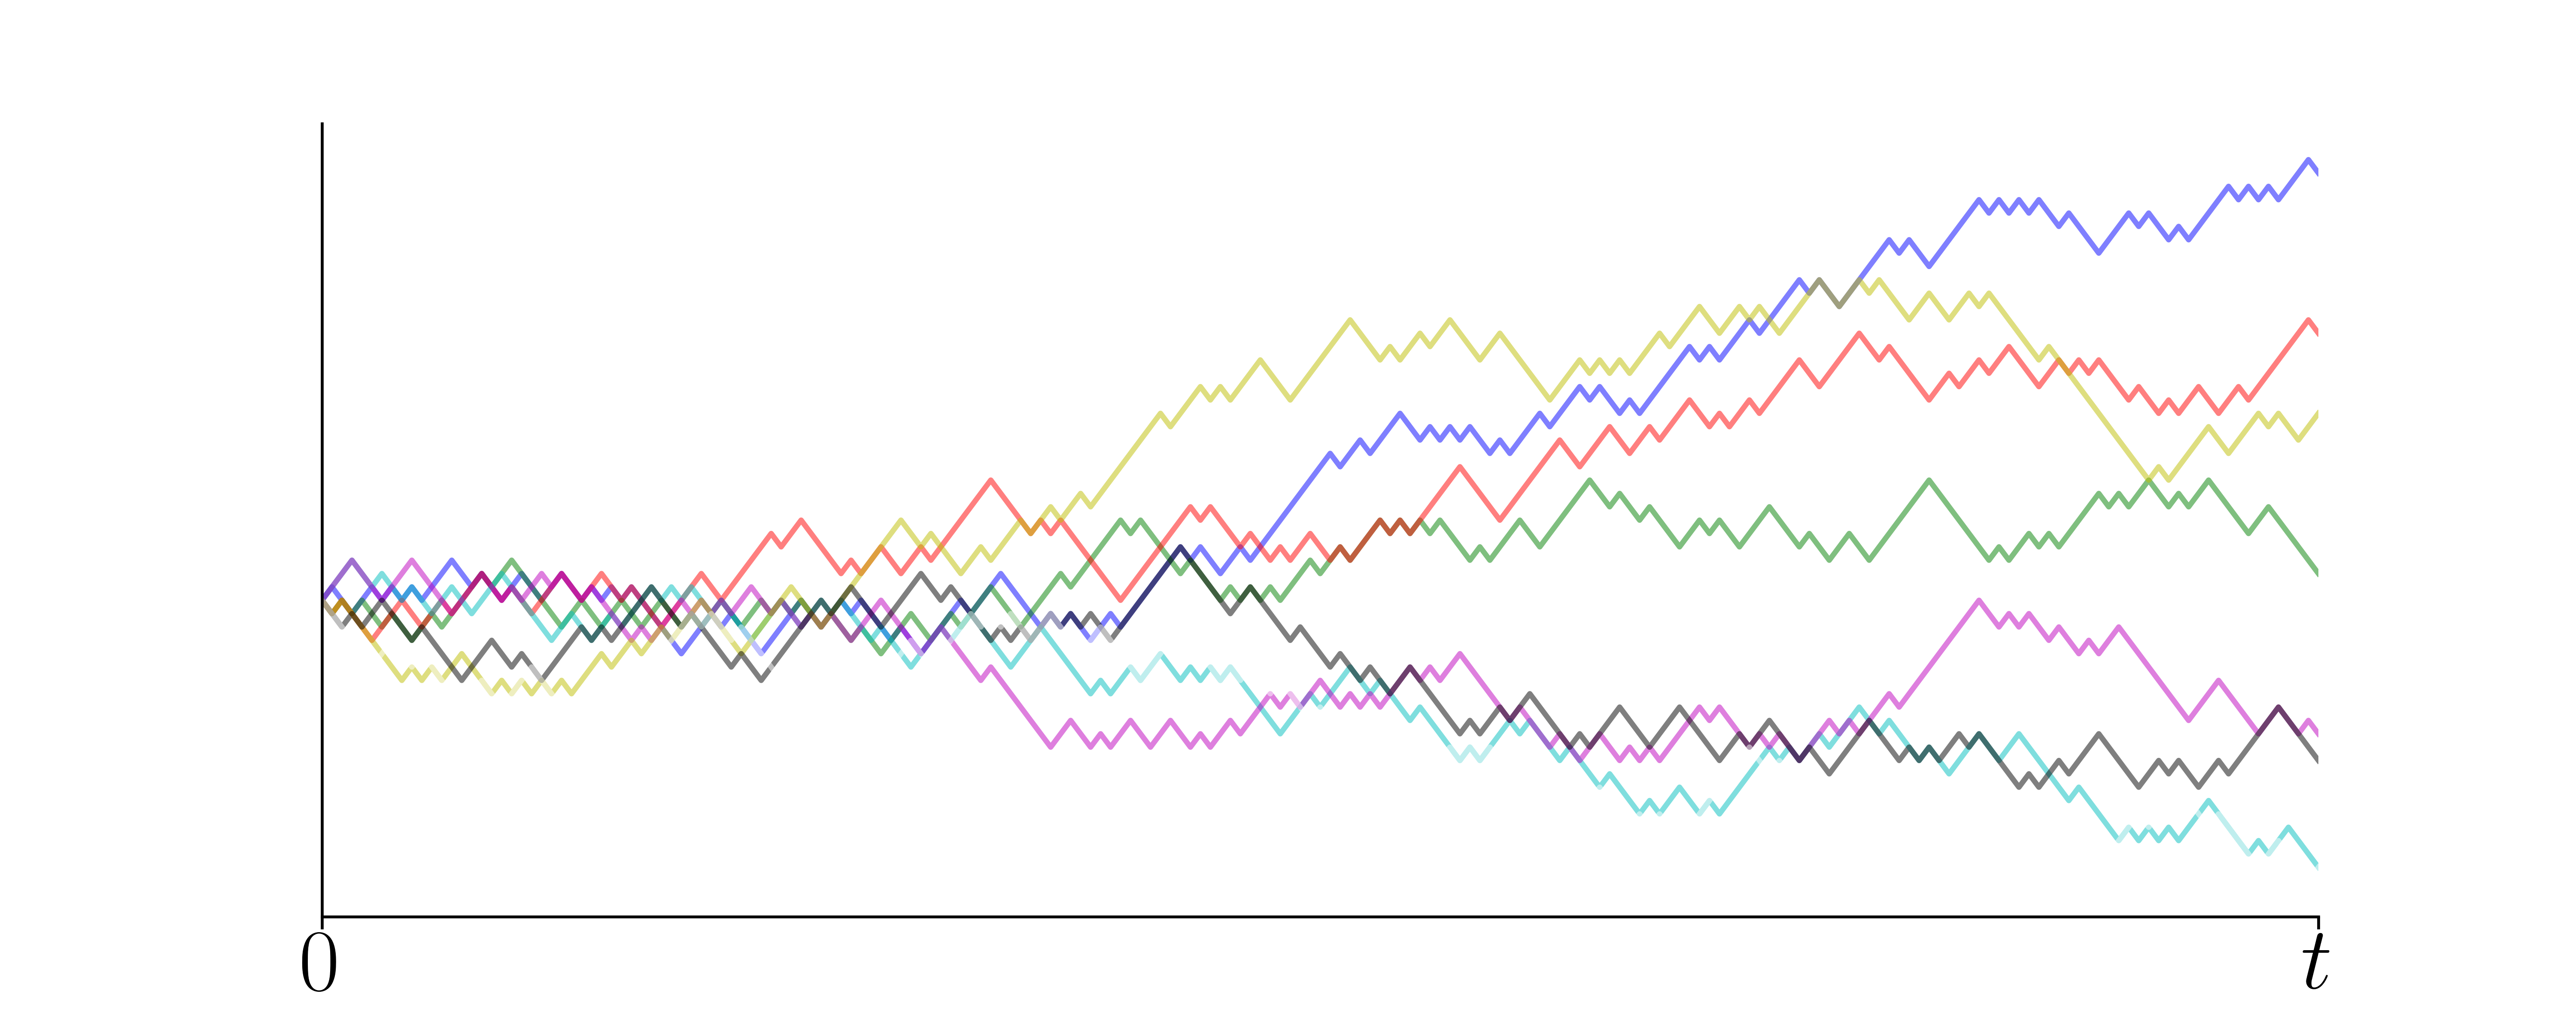
\includegraphics[width=0.95\linewidth]{Control_lecture_notes/Figs/bm_1d_100.png}
\end{frame}
\begin{frame}{Wiener process or Brownian motion}
    A Wiener process or Brownian motion is a stochastic process with the following property.
    \begin{enumerate}[label = \bfseries \arabic*)]
        \item $W_0$ is distributed according to a known distribution, $\mu$. $\mu$ can be a Dirac delta at a point, $W_0=0$.
        \item For any $t_{1}<\cdots<t_{n}$, $W_{t_{n}}-W_{t_{n-1}},...,W_{t_{2}}-W_{t_{1}}$ are independent and have Gaussian distribution with mean zero and variance $t_{n}-t_{n-1},...,t_{2}-t_{1}$.
        \item Sample paths of $W$ are continuous functions of $t$.
    \end{enumerate}
\end{frame}

\begin{frame}{Random walk}
    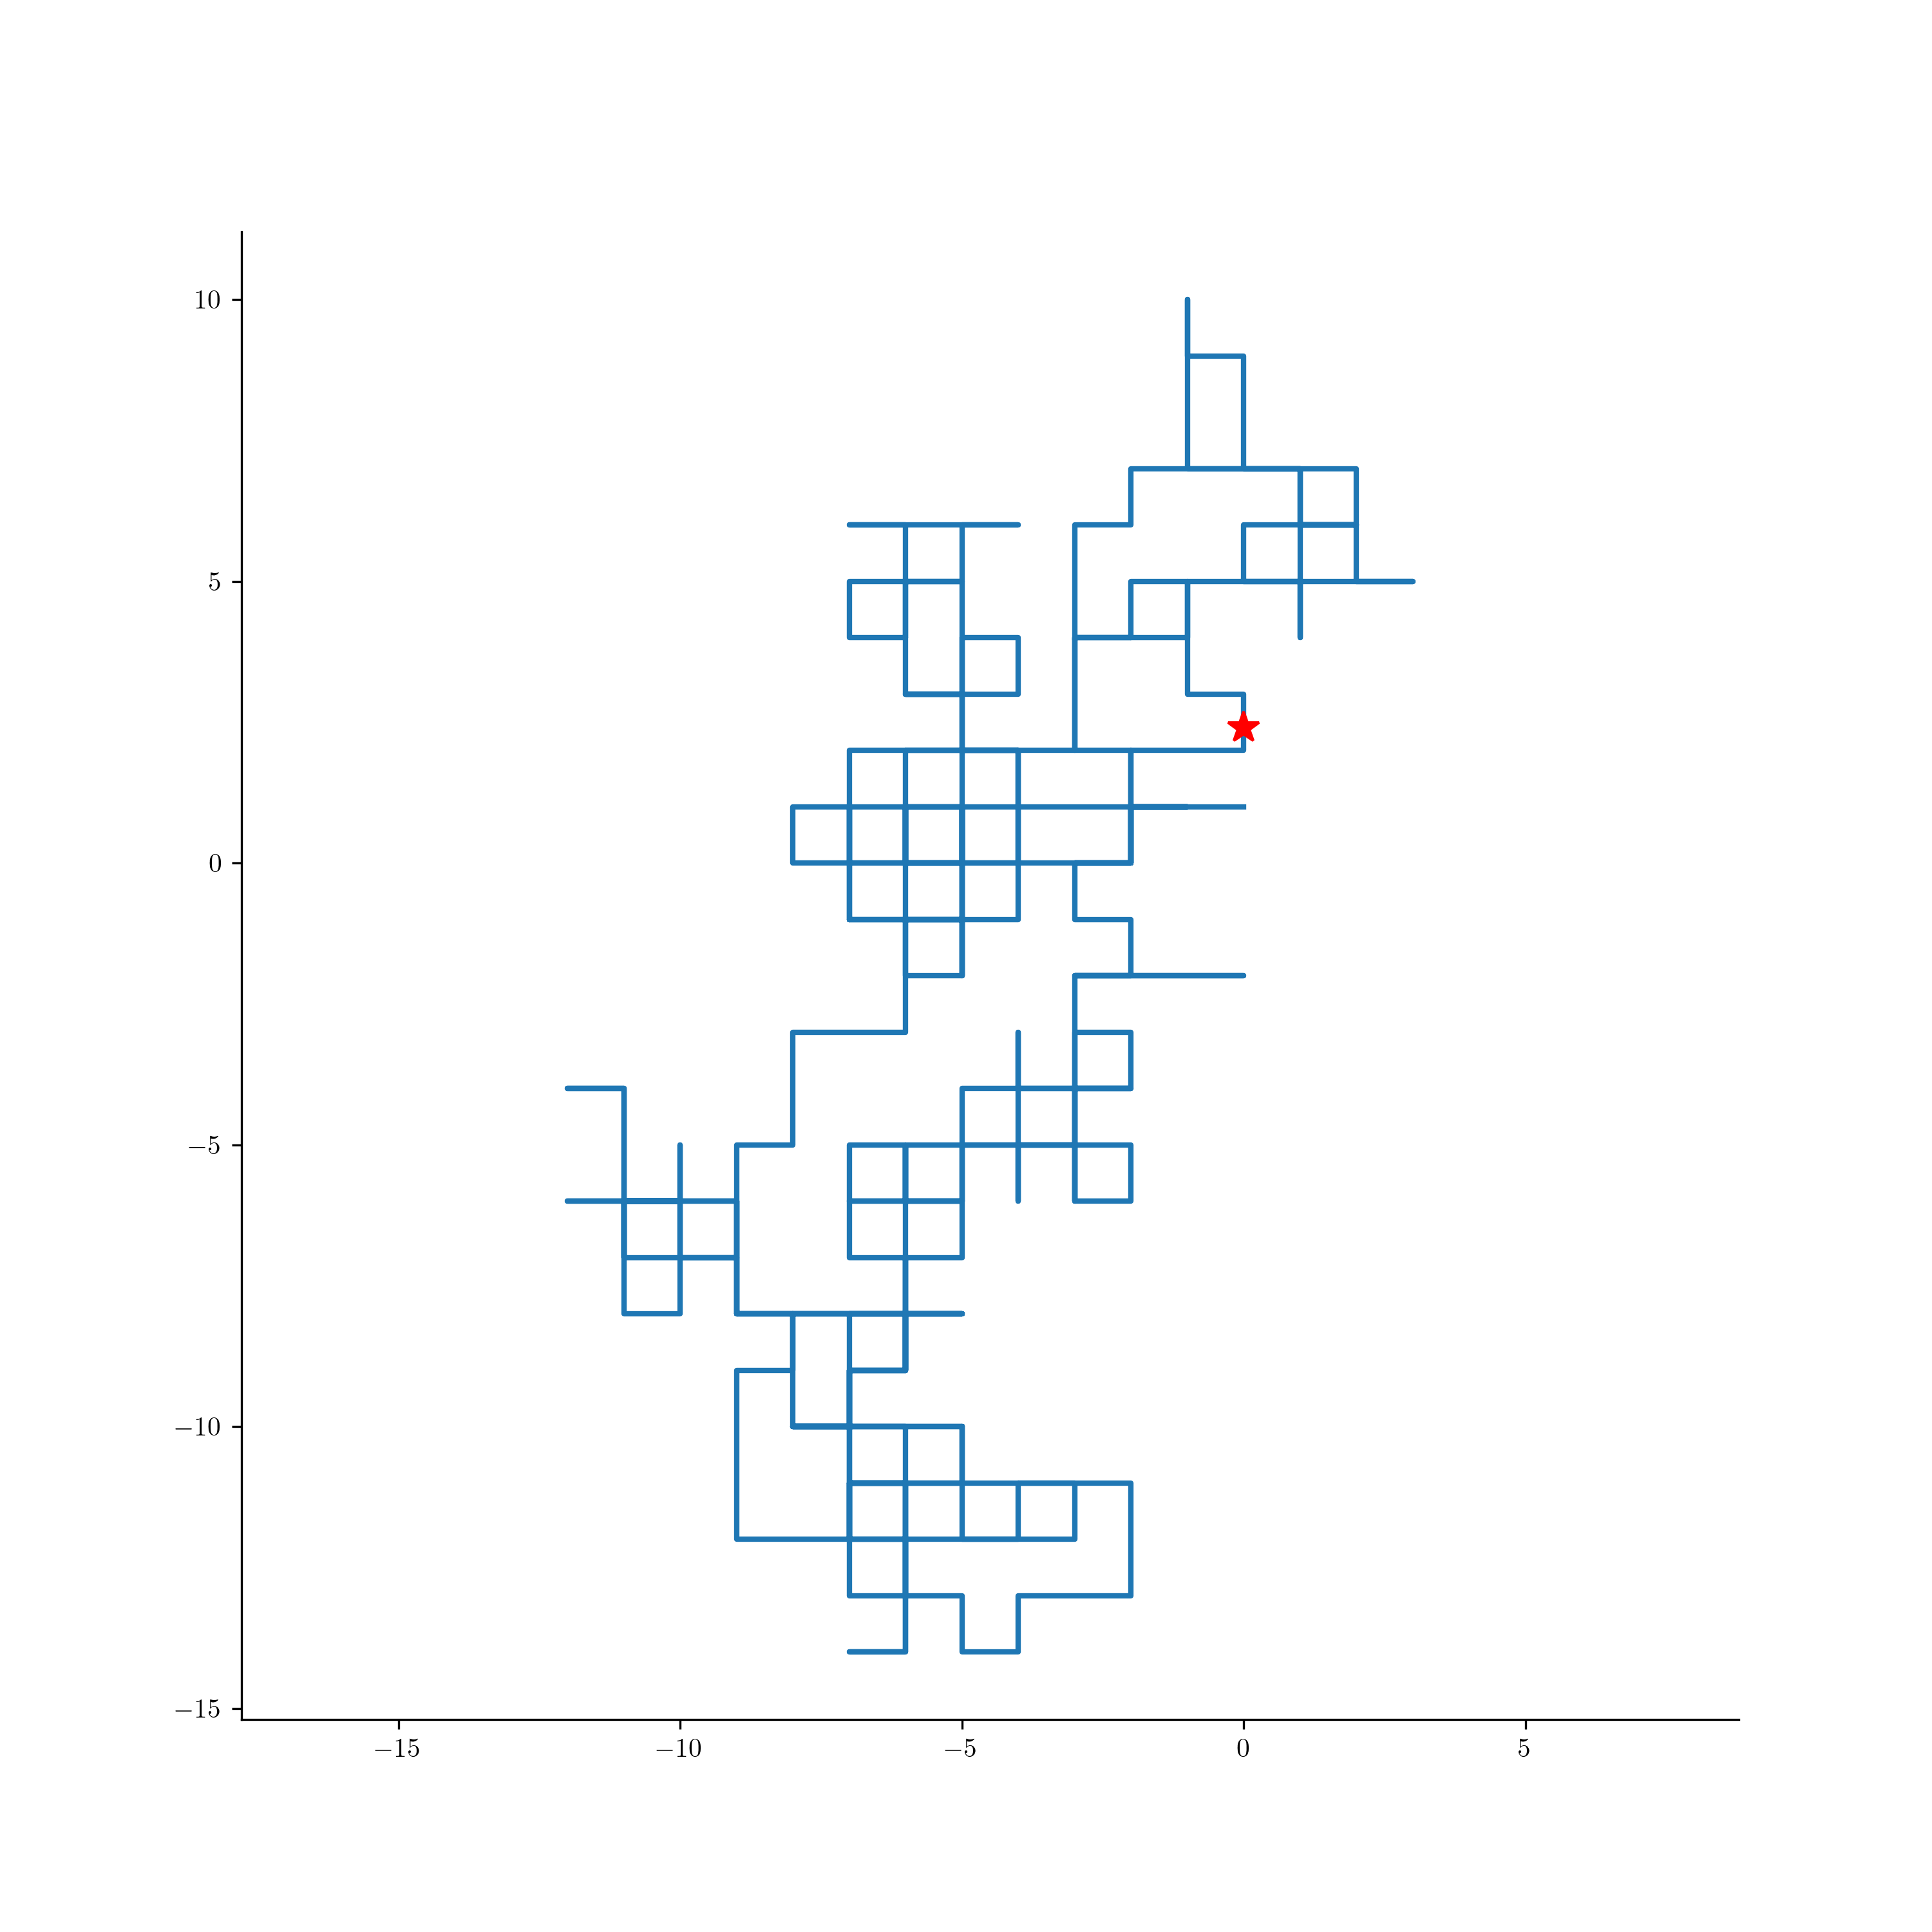
\includegraphics[width=0.75\linewidth]{Control_lecture_notes/Figs/rw_2d_1.png}
\end{frame}

\begin{frame}{Random walk to Wiener process}
    \begin{block}
        {Step size}
        For $N\in\mathbb{N}$, we modify the step size to $\sqrt{1/N}$ and modify the time between two steps by $1/N$
    \end{block}
\end{frame}

\begin{frame}{Random walk $1$}
    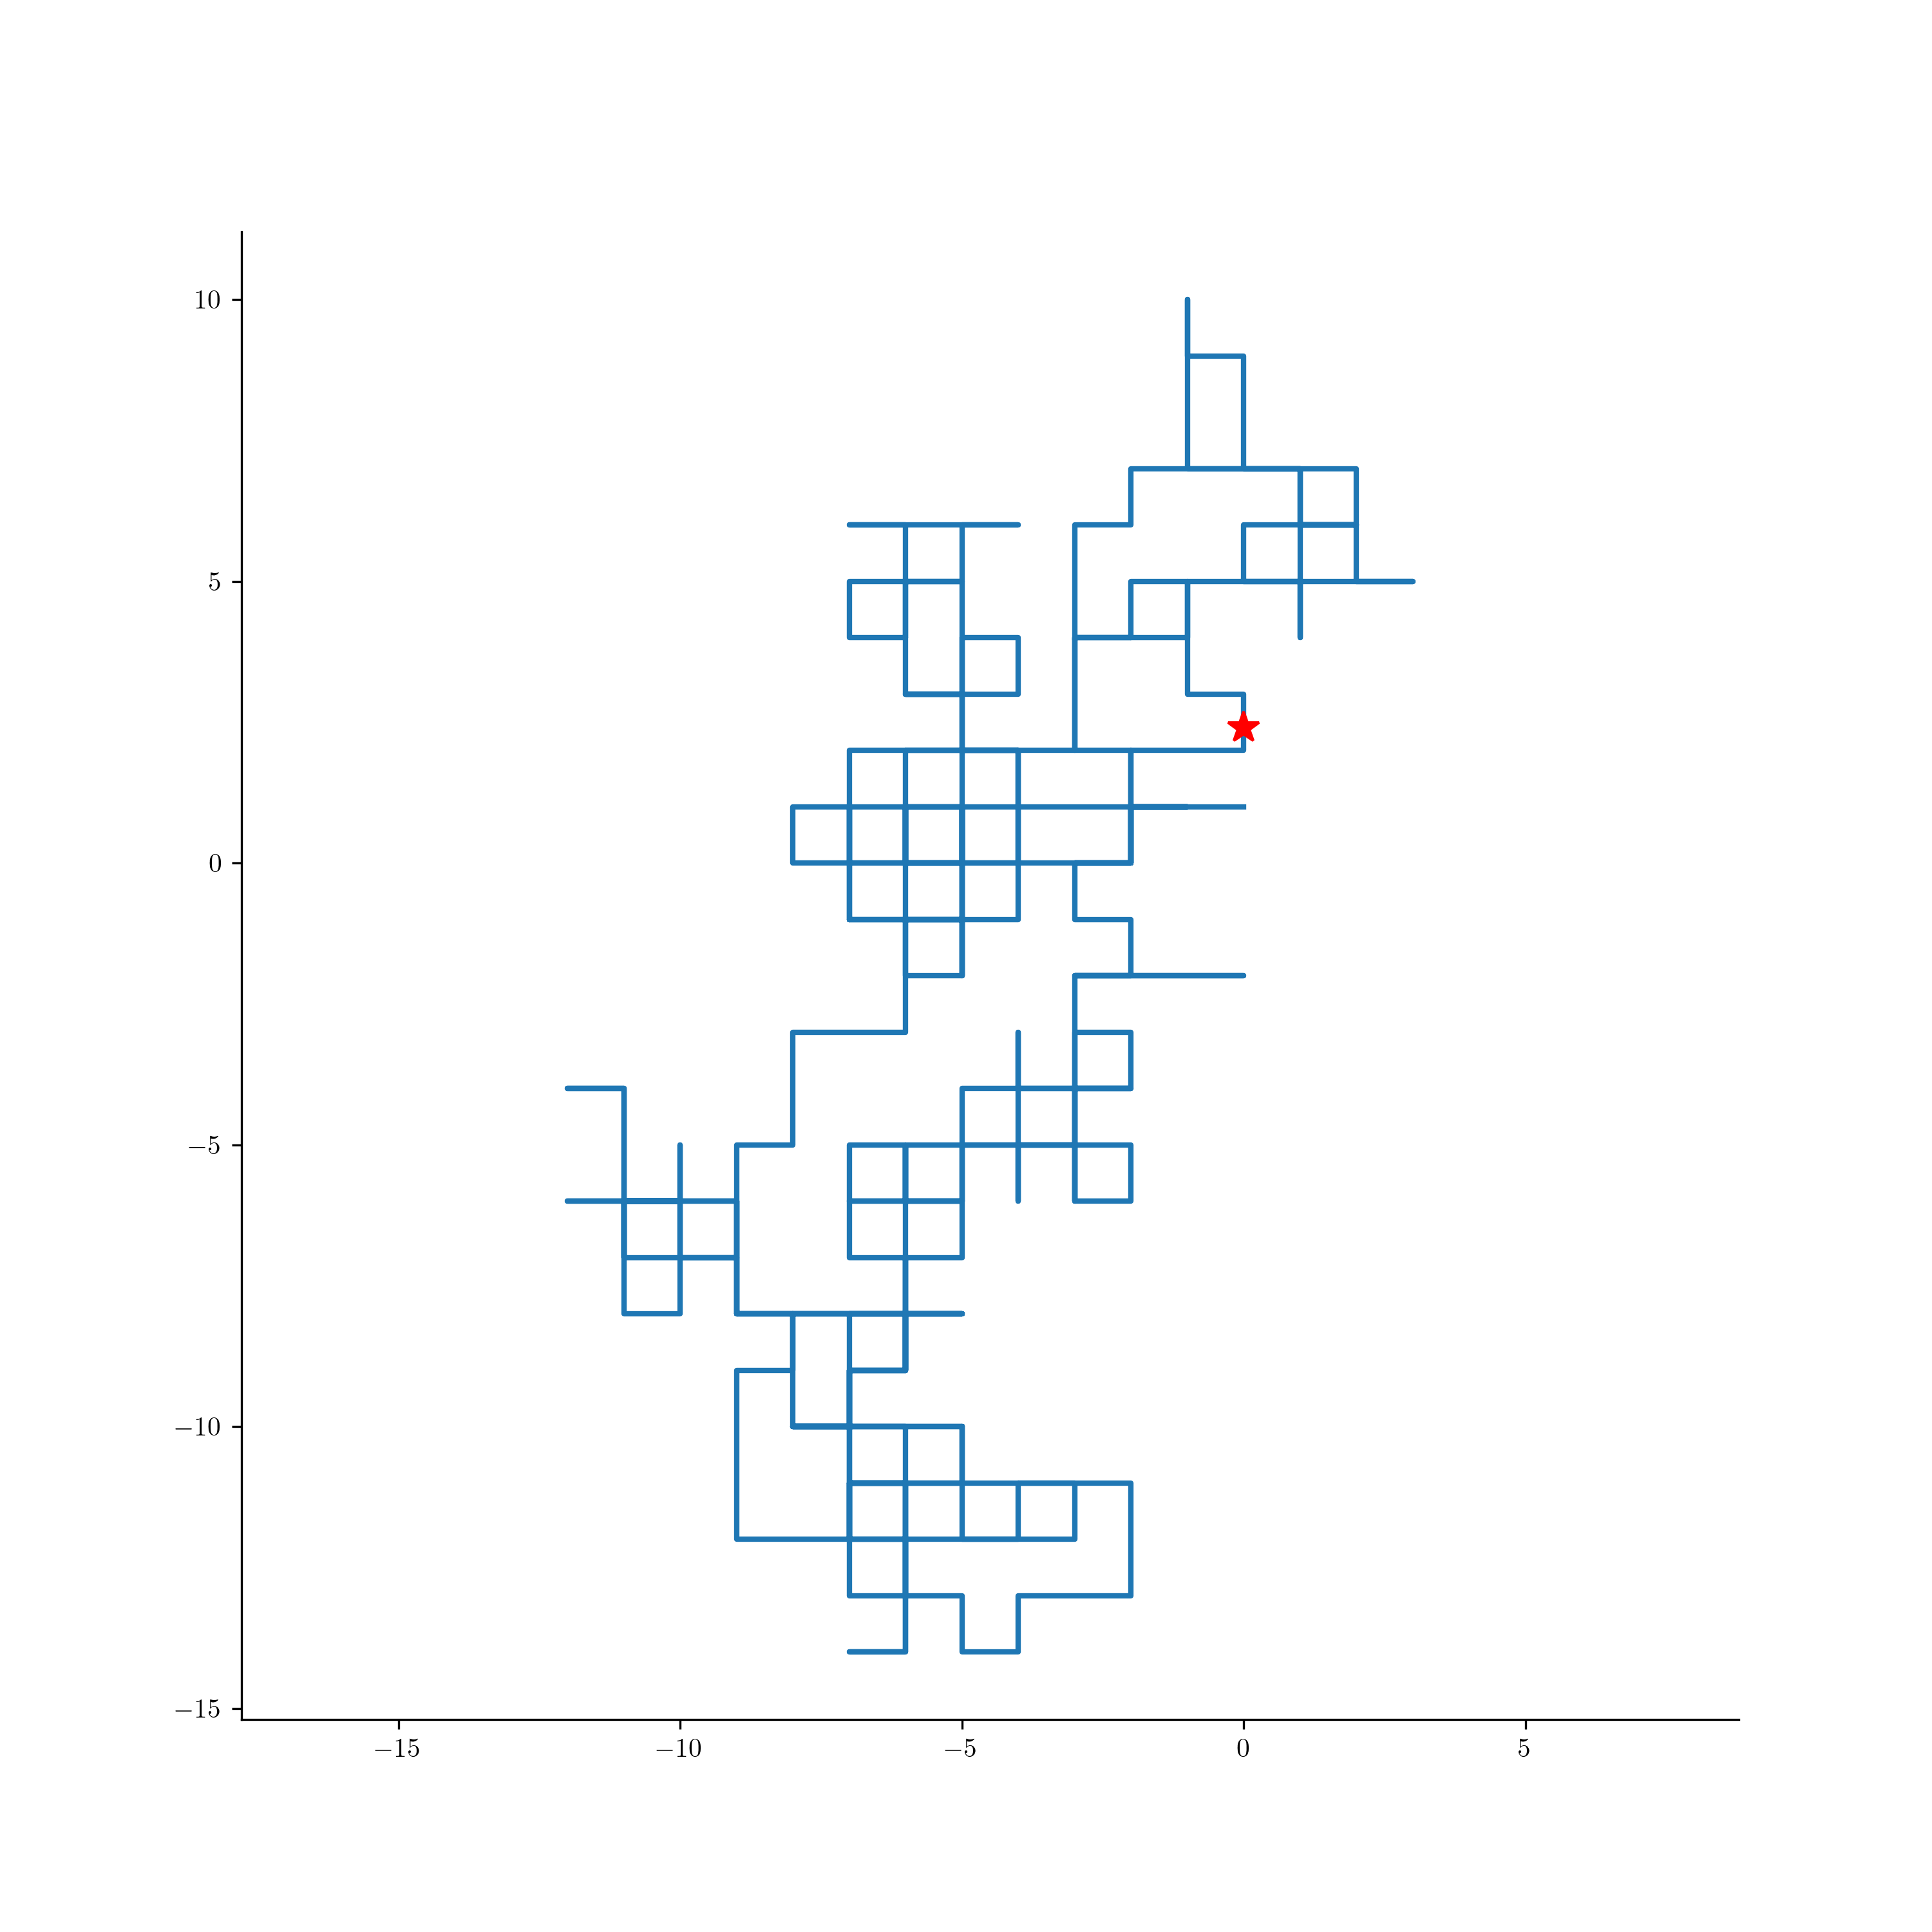
\includegraphics[width=0.8\linewidth]{Control_lecture_notes/Figs/rw_2d_1.png}
\end{frame}
\begin{frame}{Random walk $0.1$}
    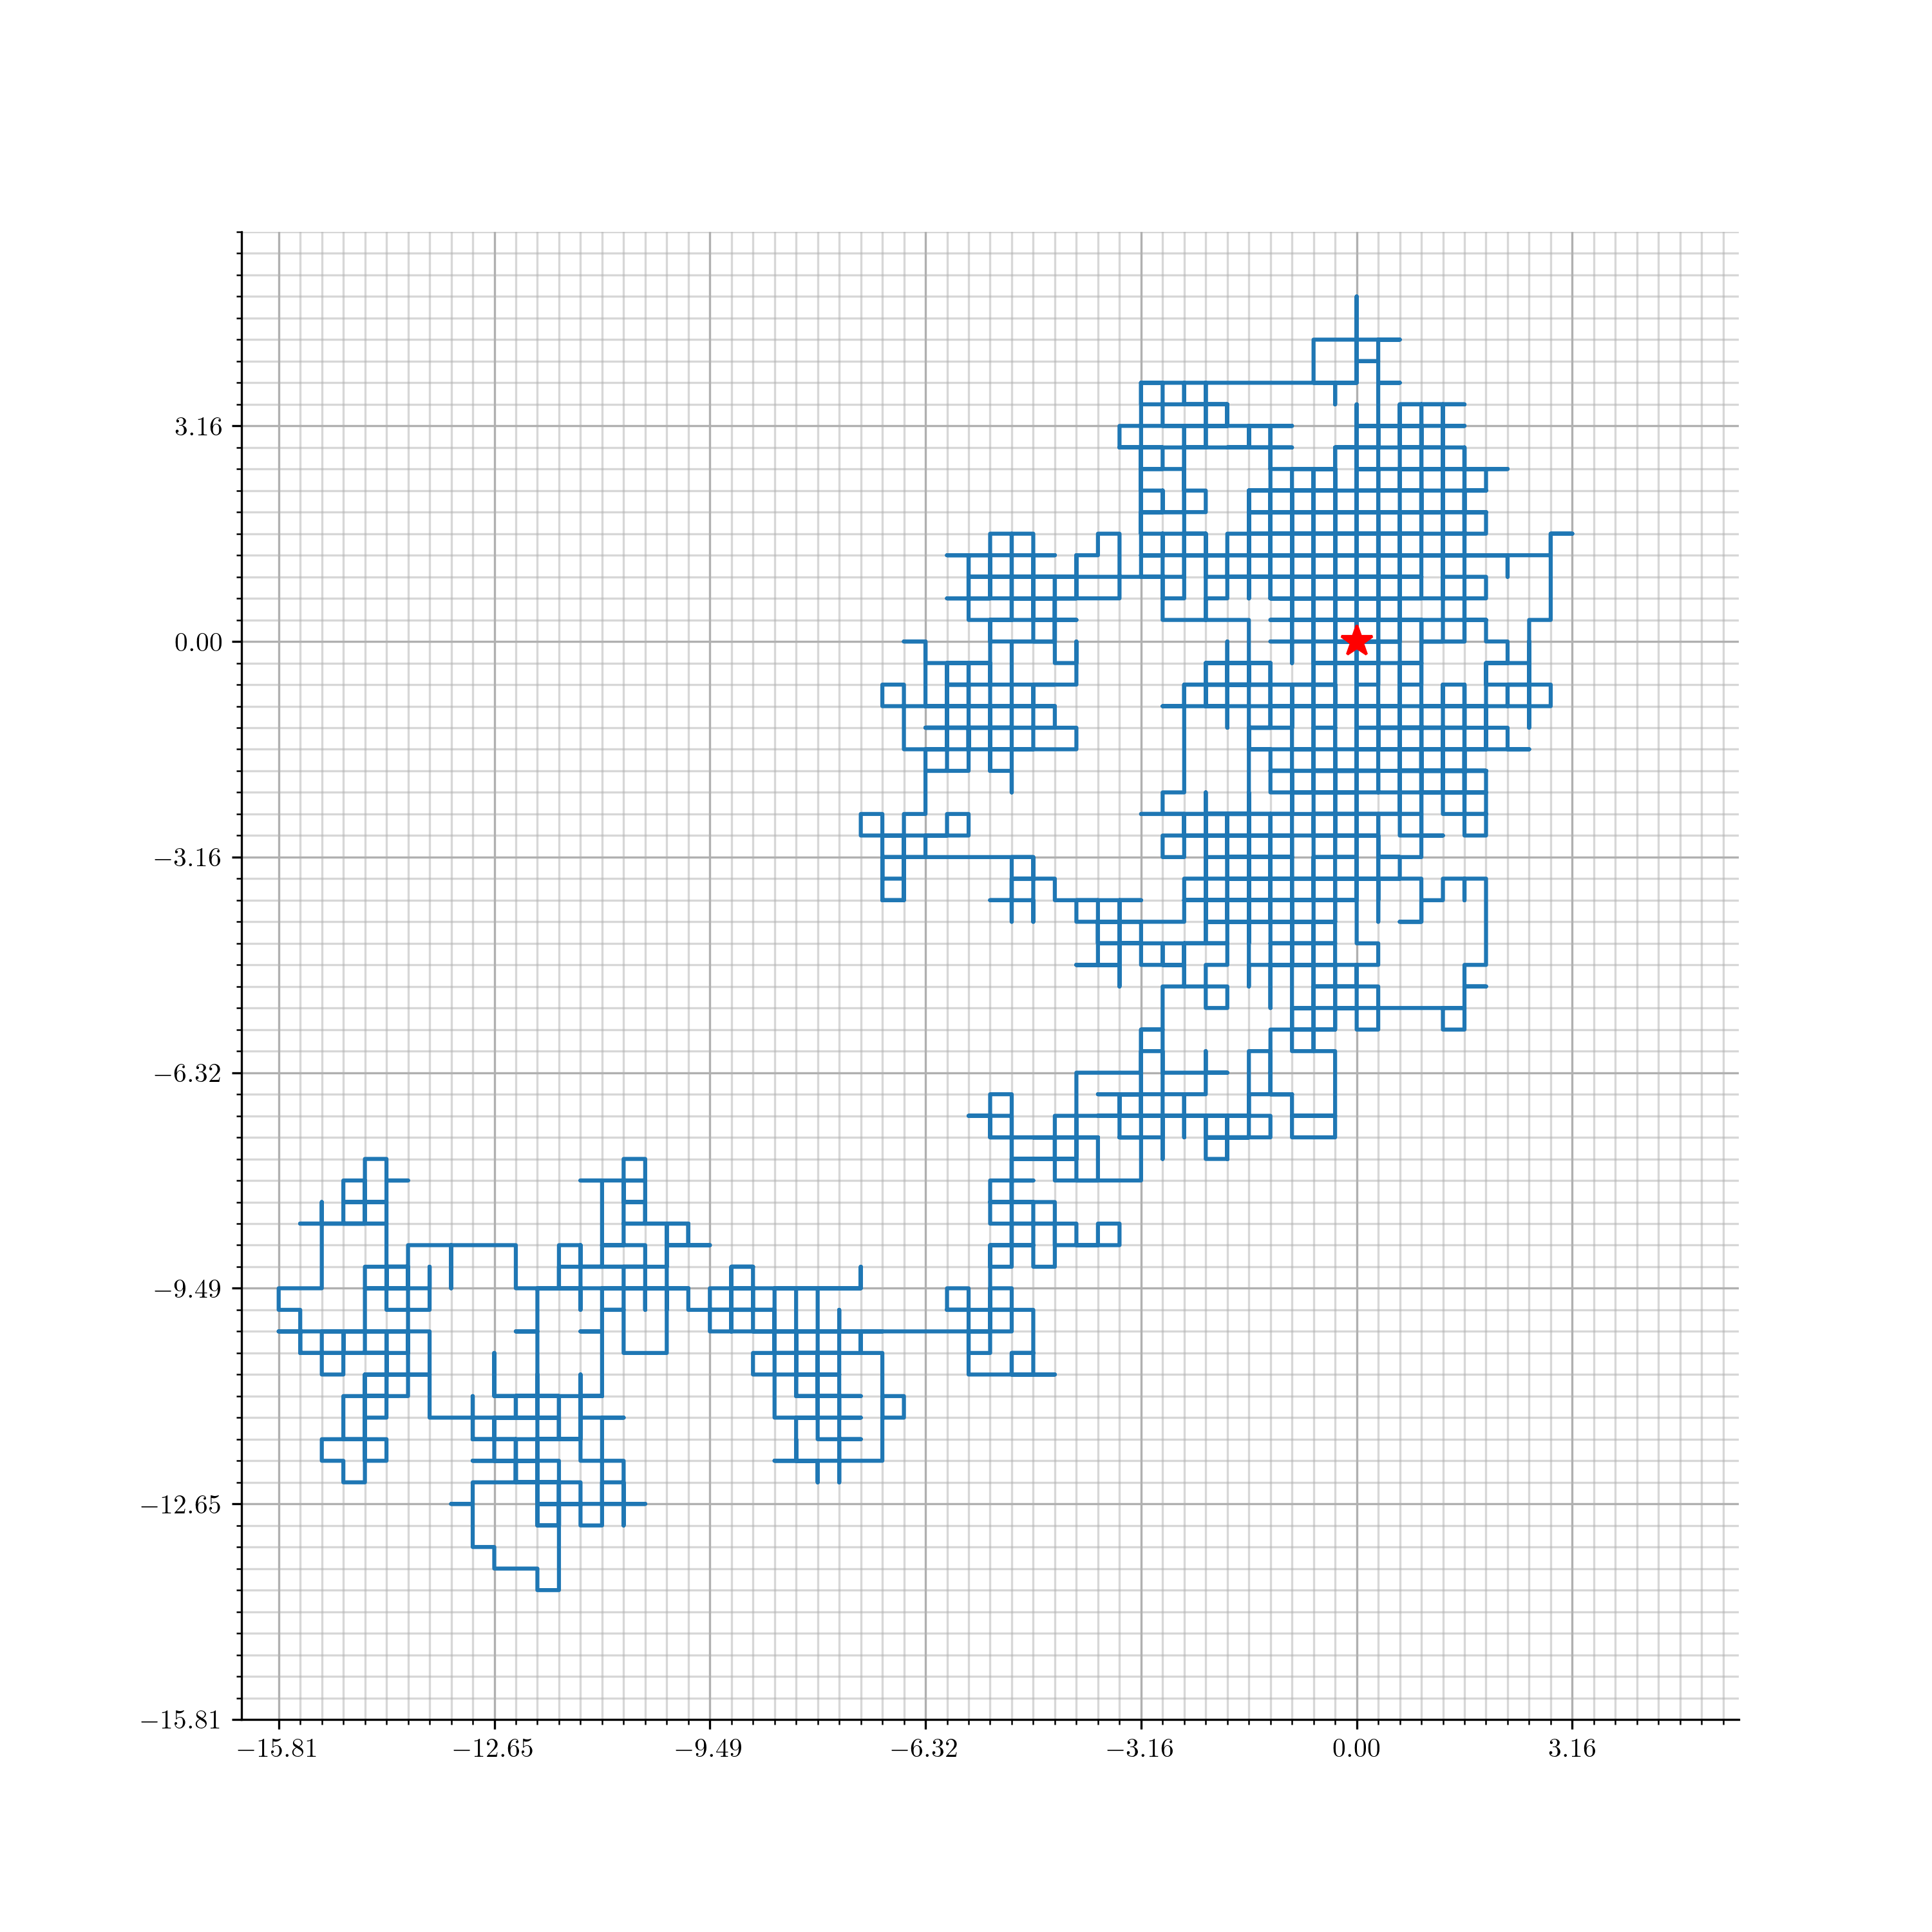
\includegraphics[width=0.8\linewidth]{Control_lecture_notes/Figs/rw_2d_10.png}
\end{frame}
\begin{frame}{Random walk $0.01$}
    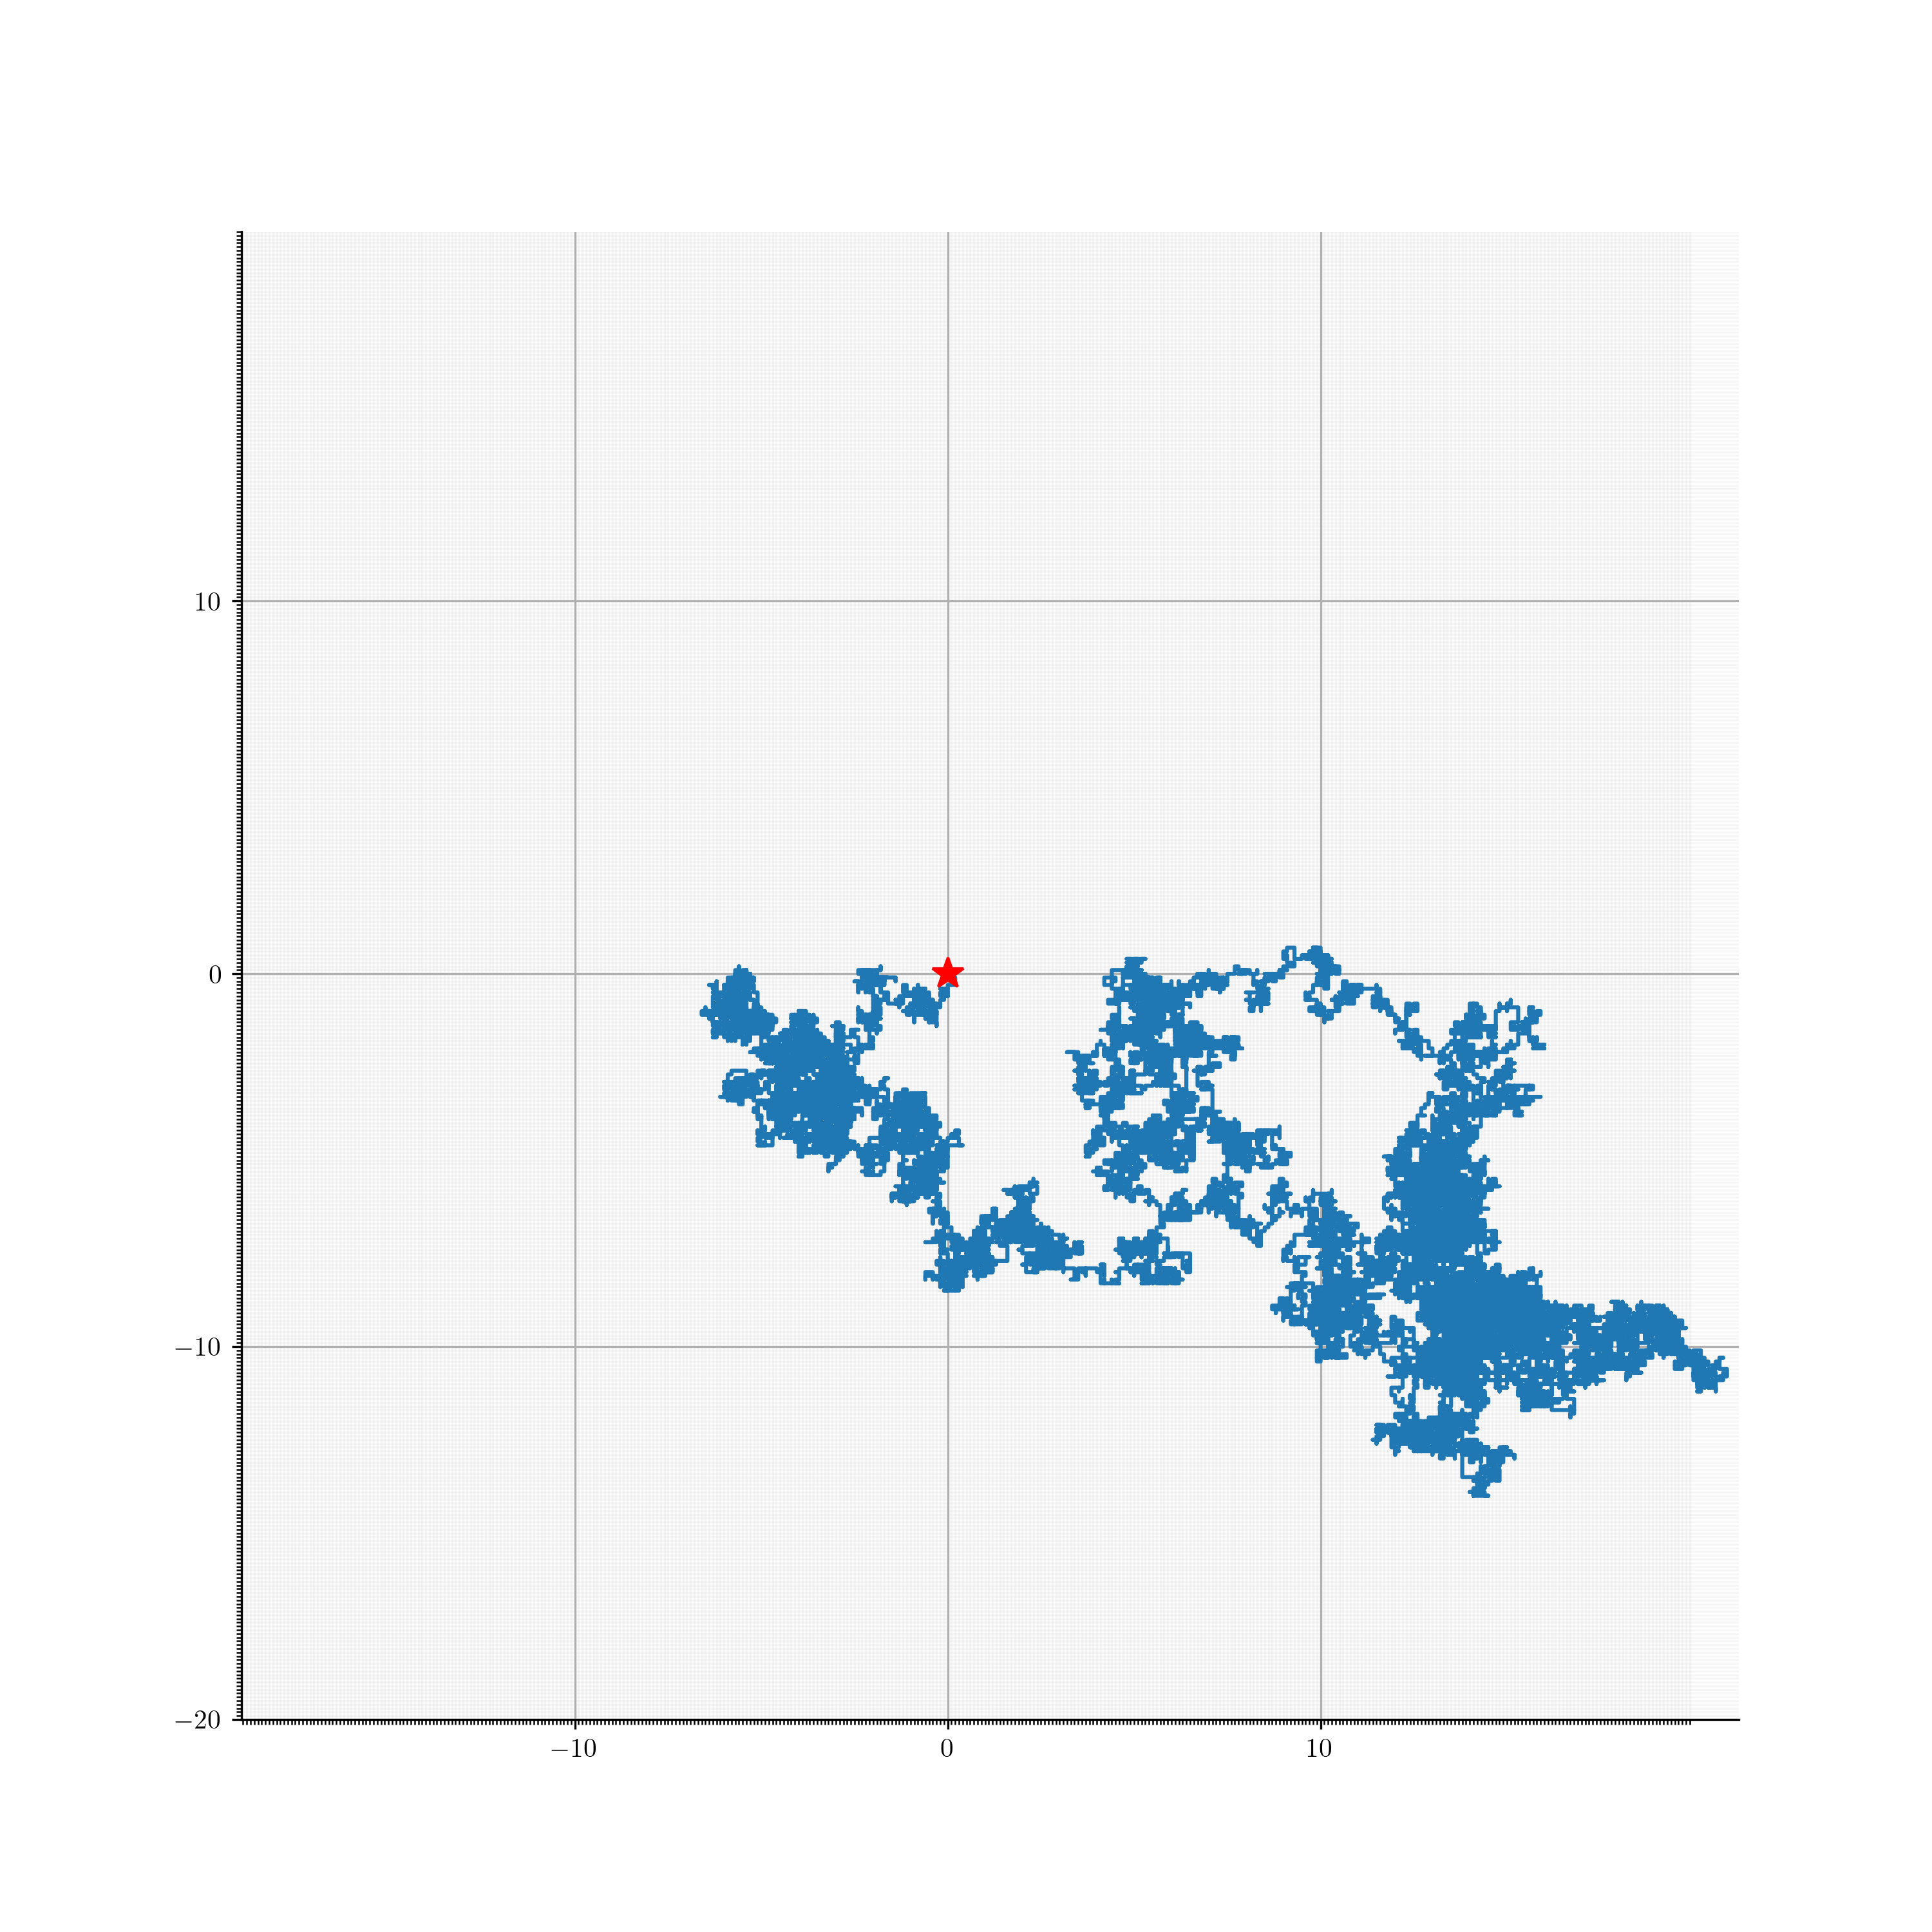
\includegraphics[width=0.8\linewidth]{Control_lecture_notes/Figs/rw_2d_100.png}
\end{frame}
\begin{frame}{Random walk $0.001$}
    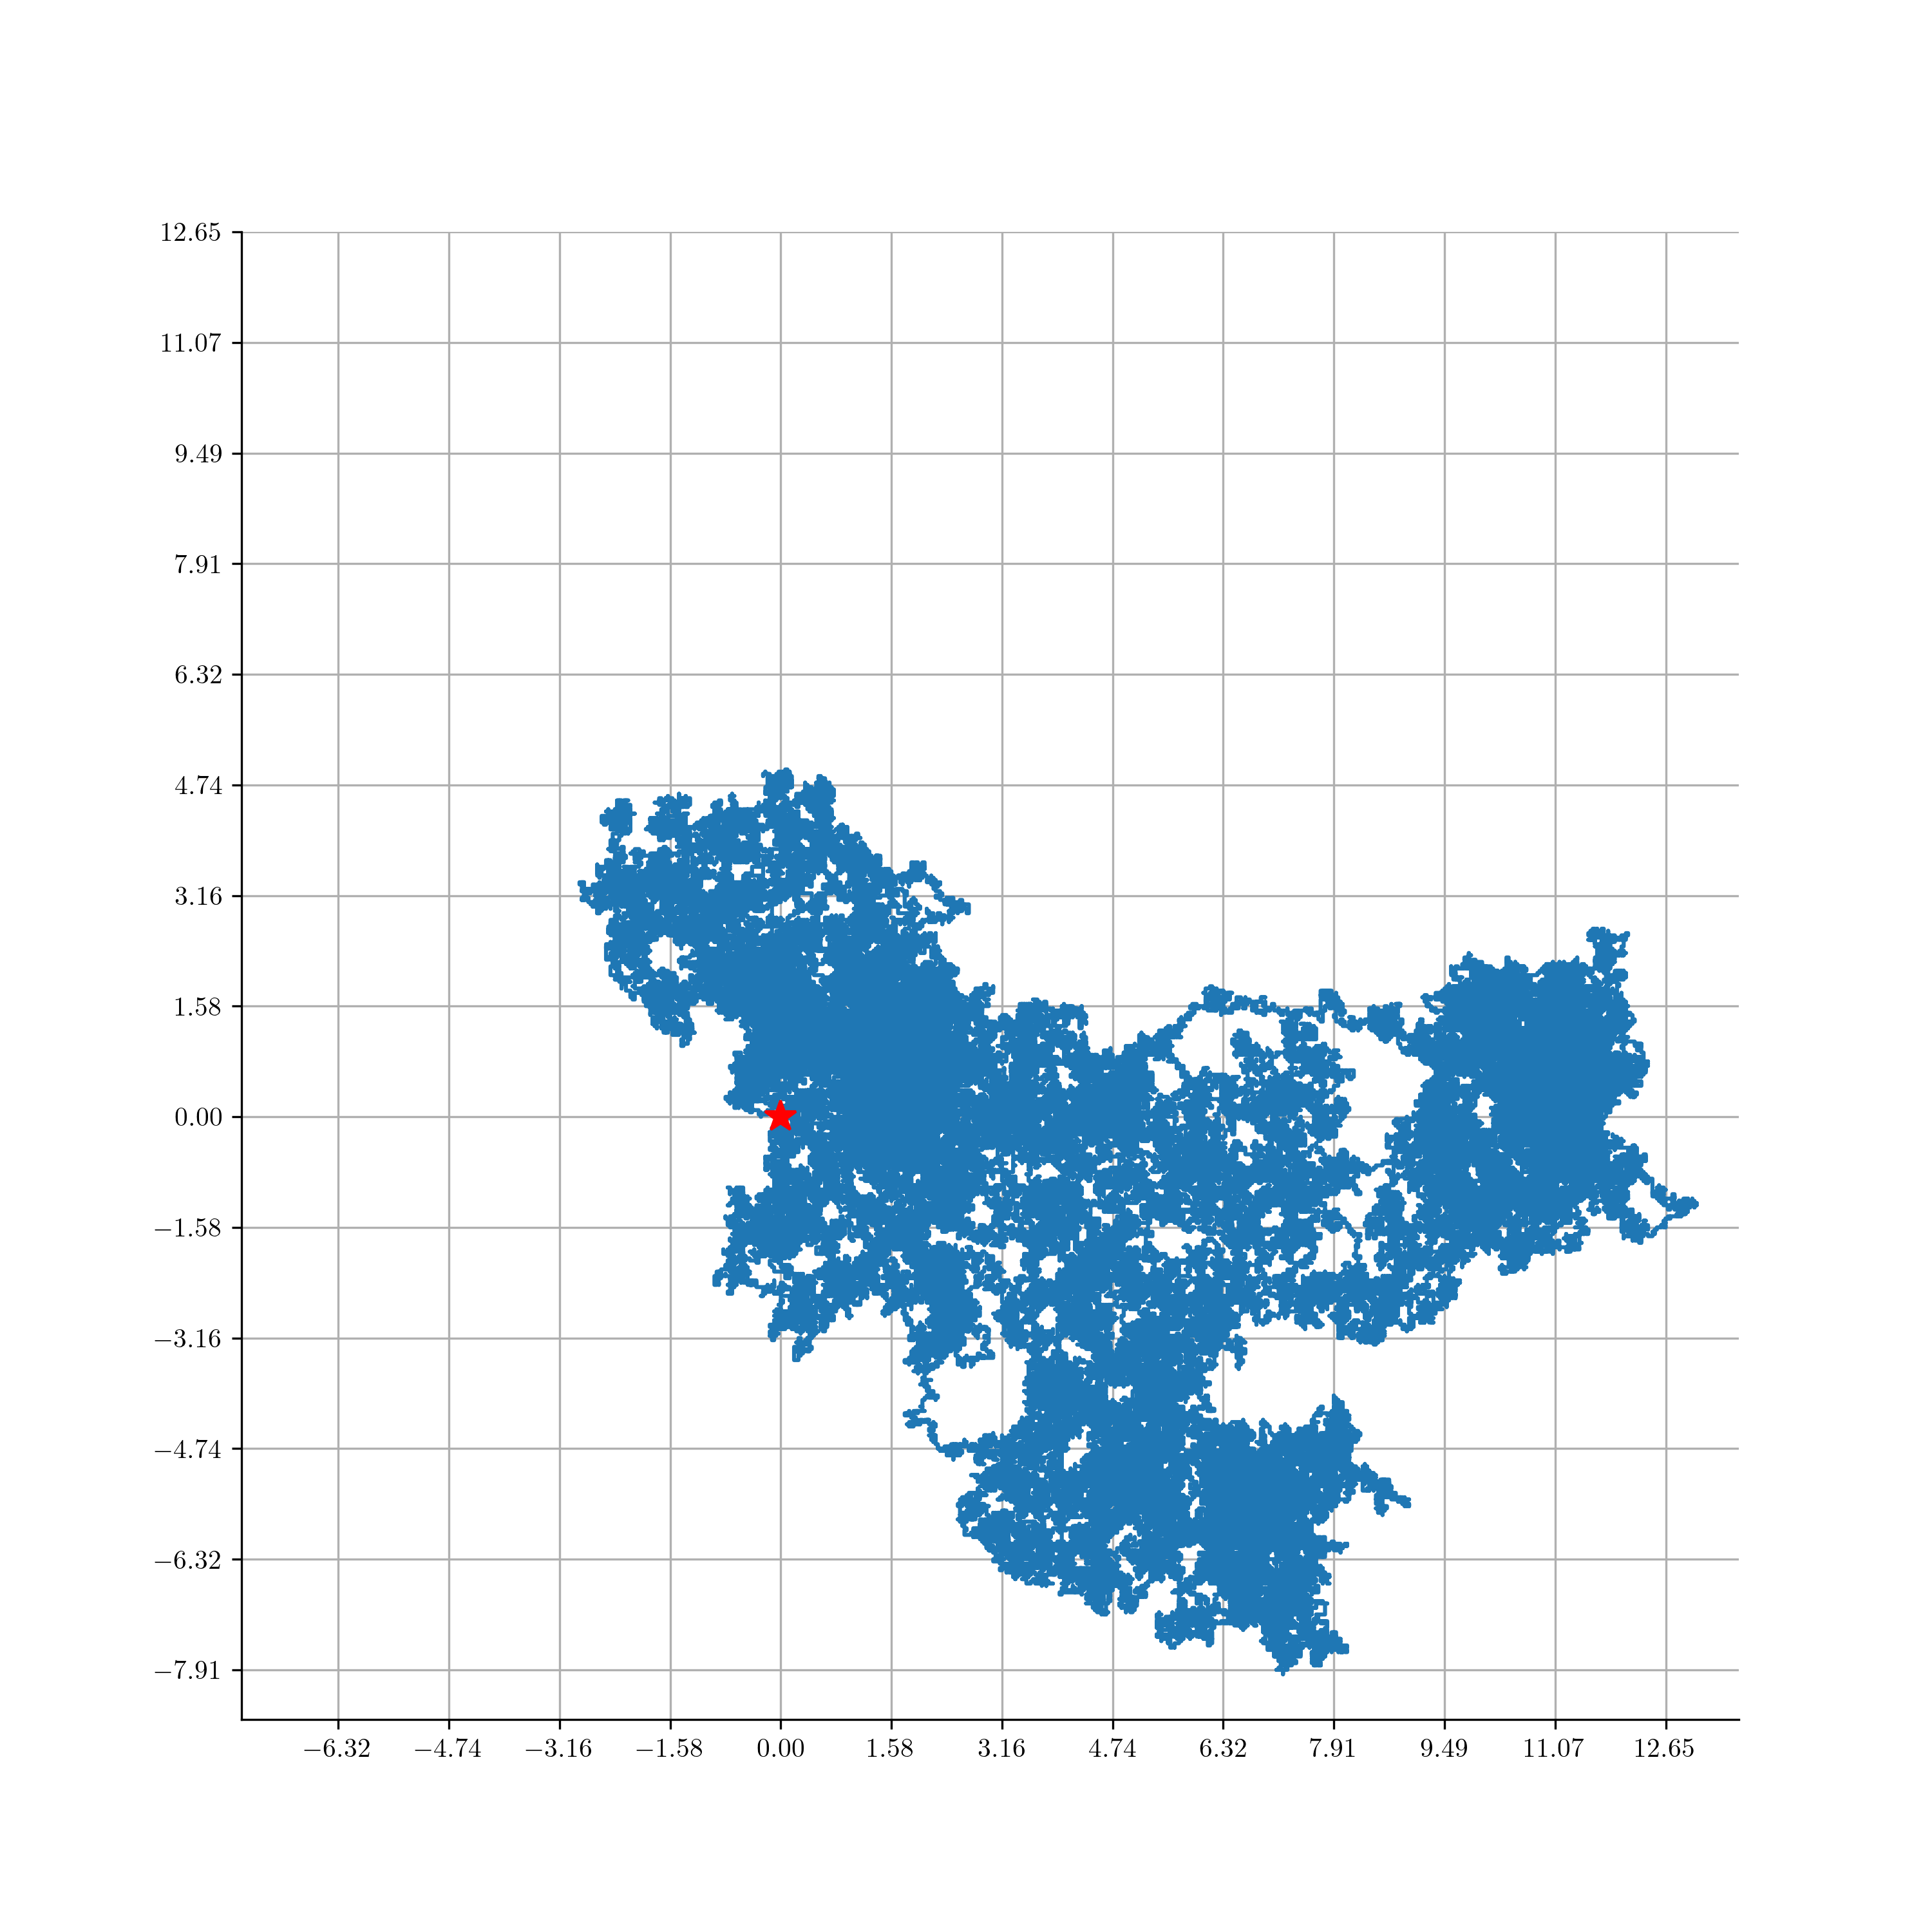
\includegraphics[width=0.8\linewidth]{Control_lecture_notes/Figs/rw_2d_1000.png}
\end{frame}
\end{document} 